\PassOptionsToPackage{pdfpagelabels=false}{hyperref}
\documentclass[fleqn,usenatbib,usedcolumn]{mnras}
%==============================================================================%
\usepackage[british]{babel}             % British English hyphenation
\usepackage{txfonts}                  % Good fonts
% Use vector fonts, so it zooms properly in on-screen viewing software
% Don't change these lines unless you know what you are doing
%\usepackage[T1]{fontenc}
%\usepackage{ae,aecompl}
%%%%% AUTHORS - PLACE YOUR OWN PACKAGES HERE %%%%%
\usepackage{graphicx}	% Including figure files
\usepackage{hyperref} % hyperlinks
\usepackage{natbib}
\usepackage{aastexmacros}
\usepackage{tikz}
\usepackage[caption=false]{subfig}
\usepackage[mediumspace,mediumqspace,Grey,squaren]{SIunits}
%%%%%%%%%%%%%%%%%%%%%%%%%%%%%%%%%%%%%%%%%%%%%%%%%%

%%%%% AUTHORS - PLACE YOUR OWN COMMANDS HERE %%%%%
\usetikzlibrary{shapes,arrows,calc,positioning}

\renewcommand{\vec}[1]{\mathbf{#1}}
% \newcommand{\text}{\mathrm}
\newcommand{\jansky}{\text{Jy}}
\newcommand{\cheng}[1]{ {\color{teal}[{\bf Cheng TODO:~{#1}}]} }
\newcommand{\matthew}[2]{ {\color{white!20!violet}[{\bf TODO(#1):~{#2}}]} }
\newcommand{\todo}[1]{ {\color{red}[{\bf TODO:~{#1}}]} }

%%%%%%%%%%%%%%%%%%%%%%%%%%%%%%%%%%%%%%%%%%%%%%%%%%

%%%%%%%%%%%%%%%%%%% TITLE PAGE %%%%%%%%%%%%%%%%%%%

\title[Machine learning methods for radio source cross-identification]{Radio Galaxy Zoo: Machine learning methods for radio source host galaxy cross-identification}

\author[Alger et al.]{
  M.~J.~Alger$^{1}$,
  J.~K.~Banfield$^{2, 1}$,
  C.~S.~Ong$^{3, 4}$,
  O.~I.~Wong$^{5, 2}$,
  L.~Rudnick$^{6}$,
  R.~P.~Norris$^{7, 8}$, others
\\
% List of institutions
$^{1}$Research School of Astronomy and Astrophysics, The Australian National University, Canberra, ACT 2611, Australia\\
$^{2}$ARC Centre of Excellence for All-Sky Astrophysics (CAASTRO)\\
$^{3}$Data61, CSIRO, Canberra, ACT 2601, Australia\\
$^{4}$Research School of Computer Science, The Australian National University, Canberra, ACT 2601, Australia\\
$^{5}$International Centre for Radio Astronomy Research-M468, The University of Western Australia, 35 Stirling Hwy, Crawley, WA 6009, Australia\\
$^{6}$Minnesota Institute for Astrophysics, University of Minnesota, 116 Church St. SE, Minneapolis, MN 55455\\
$^{7}$Western Sydney University, Locked Bag 1797, Penrith South, NSW 1797, Australia\\
$^{8}$CSIRO Astronomy \& Space Science, PO Box 76, Epping, NSW 1710, Australia
}

% These dates will be filled out by the publisher
\date{Accepted XXX. Received XXX}

% Enter the current year, for the copyright statements etc.
\pubyear{2017}

% Don't change these lines
\begin{document}
\label{firstpage}
\pagerange{\pageref{firstpage}--\pageref{lastpage}}
\maketitle

% Abstract of the paper
\begin{abstract}
  We consider the problem of determining the
  infrared host galaxies of radio emissions detected in wide-area radio
  surveys. We propose a method for reducing the cross identification task
  to binary classification, a standard machine learning task.
  Binary classification is well understood
  and well supported by machine learning software.
  We test our methods on the radio sources detected in the $1.4$~GHz
  Australian Telescope Large Area Survey (ATLAS) observations of the
  \emph{Chandra} Deep Field - South (CDFS) and the ESO Large Area ISO Survey -
  South 1 (ELAIS-S1) fields, and cross identify them with
  \emph{Spitzer} Wide-area Infrared Extragalactic survey (SWIRE).
  We compared two categories of labels:
  expert cross-identifications of CDFS from the initial ATLAS data release and
  crowdsourced cross-identifications of CDFS from Radio Galaxy Zoo.
  Our empirical results show that the cross-identification accuracy of
  the predictor trained on Radio Galaxy Zoo labels is comparable to the predictor trained
  on expert labels, demonstrating the value of crowdsourced labels.
  In addition to cross validation performance on CDFS, we demonstrate that
  our method also generalizes to ELAIS-S1.
  % We find that the best-performing expert-trained models had a mean accuracy
  % of $93.0 \pm 1.5$ per cent on CDFS and $90.4 \pm 1.5$ per cent on ELAIS-S1,
  % while the best-performing RGZ-trained models had a mean accuracy of $92.6
  % \pm 1.9$ per cent on CDFS and $88.3 \pm 0.8$ per cent on ELAIS-S1. While
  % expert-trained models outperformed models trained on the Radio Galaxy Zoo
  % labels by up to $4.3 \pm 1.1$ percentage points on CDFS and $9.1 \pm 0.9$
  % percentage points on ELAIS-S1, these models were generally comparable and
  % the crowdsourced labels hence provide a valuable training set for future
  % machine learning methods.
  Cross-identification performance with our method is limited by a lack of
  radio morphology information as our method for reducing cross identification
  to binary classification require that radio sources
  are isolated from other sources. This assumption breaks down particularly
  with high surface brightness sensitivity surveys. We suggest that source
  identifications and radio morphology information would resolve this problem.
\end{abstract}

% Select between one and six entries from the list of approved keywords.
% Don't make up new ones.
\begin{keywords}
galaxies: active -- galaxies: clusters -- radio continuum: galaxies
\end{keywords}

%%%%%%%%%%%%%%%%%%%%%%%%%%%%%%%%%%%%%%%%%%%%%%%%%%
%%%%%%%%%%%%%%%%% BODY OF PAPER %%%%%%%%%%%%%%%%%%

\section{Introduction}\label{introduction}

  Next generation radio telescopes such as the Australian SKA Pathfinder
  \citep[ASKAP;][]{johnston07} and Apertif \citep{verheijen08} will conduct
  increasingly wide, deep, and high-resolution radio surveys, producing large
  amounts of data. The Evolutionary Map of the Universe survey
  \citep[EMU;][]{norris11} using ASKAP and the WODAN survey
  \citep{rottgering11} using Apertif are expected to detect over 100 million
  radio components between them, compared to the 2.5 million radio components
  already known \citep{banfield15}.

  An important part of processing this data is cross-identifying observed
  radio emission regions with observations of their host galaxy in surveys at
  other wavelengths. Radio host cross-identification can be a difficult task.
  \autoref{fig1} illustrates the different radio emission regions that a host
  galaxy may have. Compact components are unresolved or point-like regions of
  radio emission while compact radio sources are one compact component usually
  consistent with the host galaxy location. Extended radio sources consist of
  resolved single components and/or multiple or resolved or unresolved
  components. Fanaroff \& Riley type I \citep[FRI; ][]{Fanaroff1974} and
  Fanaroff \& Riley type II (FRII) are examples of resolved radio sources.
  Radio emissions from radio-loud active galactic nuclei (AGN) may be
  complicated structures not clearly related to the host galaxy. These are
  often composed of multiple, separate components. This type of AGN are
  expected to dominate approximately 30 per cent of sources detected by EMU
  \citep{norris11}. Small surveys of a few thousand sources such as the
  Australia Telescope Large Area Survey
  \citep[ATLAS;][]{norris06,middelberg08} can be cross-identified manually,
  but this is impractical for larger surveys.

  One approach to cross-identification is crowdsourcing, where volunteers
  cross-identify radio components (both resolved and unresolved; see
  \autoref{fig1}) with their host galaxy. This is the premise of Radio Galaxy
  Zoo\footnote{\url{https://radio.galaxyzoo.org}} \citep{banfield15}, a
  citizen science project hosted on the highly successful Zooniverse platform
  \citep{lintott08}. Volunteers are shown images of the radio sky, and are
  asked to identify the radio components in each image that correspond to the
  same host galaxy. They are then asked to cross-identify the radio source
  with its host galaxy in a corresponding infrared image. A more thorough
  explanation of the project can be found in \citet{banfield15}. The first
  data release for Radio Galaxy Zoo will provide a large dataset of over
  75~000 radio host cross-identifications and radio source morphologies
  \citep{wong17}. While this is a much larger number of visual
  cross-identifications than have been made by experts \citep[e.g.,
  ][]{Taylor2007,Gendre2008,Grant2010,norris06,middelberg08} it is still far
  short of the millions of radio sources expected to be detected in upcoming
  radio surveys.

  Automated algorithms have been developed for this cross-identification
  problem. \citet{fan15} developed a method of cross-identification using
  Bayesian hypothesis testing, fitting a three-component model to extended
  radio sources. This was achieved under the assumption that extended radio
  sources are composed of a core radio component and two lobe components. The
  core radio component is coincident with the host galaxy, so
  cross-identification amounts to finding the galaxy coincident with the core
  radio component in the most likely model fit. This method is easily extended
  to use other, more complex models, but it is purely geometric. The model
  does not incorporate other information such as the physical properties of
  the potential host galaxy. Additionally, there may be new classes of radio
  sources detected in future surveys like EMU which do not fit the model.
  \citet{weston17} developed a modification of the likelihood ratio method of
  cross-identification \citep{richter75likelihood} for application to ATLAS
  and EMU. This method does well on single (resolved or compact) radio sources
  with a 69 and 71 per cent success rate in the two ATLAS fields, but does not
  currently handle extended multiple component radio sources
  \citep{norris17unexpected}. A hope is that machine learning techniques can
  be developed for cross-identification problem. Machine learning describes a
  class of methods that learn approximations to functions, and so if the
  cross-identification task can be cast as a machine learning problem, data
  sets such as that provided by Radio Galaxy Zoo can be generalised to work on
  data unseen by the original cross-identifiers.

  We have developed a machine learning approach for radio host
  cross-identification. This approach casts the cross-identification task as
  binary classification, which is very well-understood in machine learning
  literature and can be solved using a variety of standard, well-known
  techniques. We have trained these methods on expert cross-identifications
  and cross-identifications from Radio Galaxy Zoo. In \autoref{sec:data} we
  describe the data we use to train our methods. In \autoref{sec:method} we
  discuss how we cast the radio host galaxy cross-identification problem as a
  machine learning problem. In \autoref{sec:results} we present results of
  applying our method to ATLAS observations of the \emph{Chandra} Deep Field -
  South (CDFS) and in \autoref{sec:elais} we apply the cross-identifiers
  trained on CDFS to the ESO Large Area ISO Survey - South 1 (ELAIS-S1) field.
  Our data and code are available at
  \url{https://radiogalaxyzoo.github.io/atlas-xid}.

  \begin{figure}
  \begin{center}
    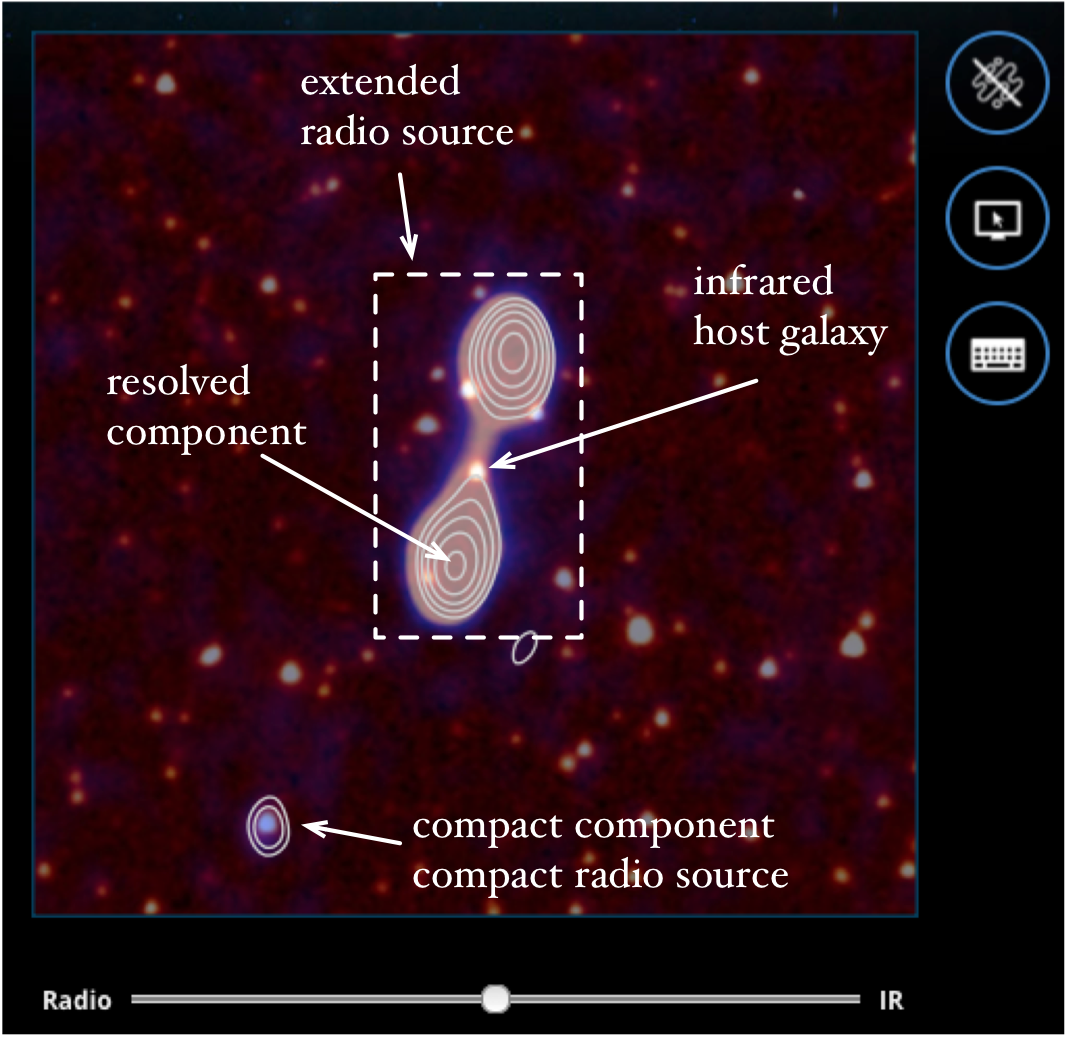
\includegraphics[width=0.75\linewidth]{images/fig1.png}
    \caption{The Radio Galaxy Zoo tutorial image illustrating key definitions
      used throughout this paper. A colour version of this figure is available
      online.}\label{fig1}
  \end{center}
  \end{figure}

\section{Data}\label{sec:data}

  We use data from the citizen science project Radio Galaxy Zoo
  \citep{banfield15}, the Australia Telescope Large Area Survey
  \citep[ATLAS;][]{norris06,franzen15}, and the \emph{Spitzer} Wide-area Infrared
  Extragalactic survey \citep[SWIRE;][]{lonsdale03swire, surace05swire}.

  \subsection{ATLAS}\label{sec:atlas}
    \begin{table}
      \caption{Catalogues of ATLAS/SWIRE cross-identifications for the CDFS
        and ELAIS-S1 fields. The method used to generate each catalogue is
        shown, along with the number of radio components cross-identified in each
        field.}
      \label{tab:atlas-cids}
      \begin{tabular}{llcc}
        \hline
        Catalogue & Method & CDFS & ELAIS-S1\\
         % & & components & components\\
        \hline
        \citet{norris06} & Manual & 784 & 0\\
        \citet{middelberg08} & Manual & 0 & 1366\\
        \citet{fan15} & Bayesian models & 784 & 0\\
        \citet{wong17} & Crowdsourcing & 2460 & 0 \\
        \citet{weston17} & Likelihood ratio & 3078 & 2113\\
        \hline
      \end{tabular}
    \end{table}

    ATLAS is a pilot survey for the EMU \citep{norris11} survey, which will
    cover the entire southern sky and is expected to detect approximately 70
    million new radio sources. EMU will be conducted at the same depth and
    resolution as ATLAS, so methods developed for processing ATLAS data are
    expected to work for EMU. ATLAS is a wide-area radio survey of the CDFS
    and ELAIS-S1 fields at 1.4~GHz with a sensitivity of
    14 and \unit{17}{\micro\jansky} on CDFS and ELAIS-S1 respectively.
    CDFS covers 3.6~deg$^2$ and contains 3034 radio components above
    5$\sigma$. ELAIS-S1 covers 2.7~deg$^2$ and contains 2084 radio components
    above 5$\sigma$ \citep{franzen15}. A number of catalogues have been
    produced cross-identifying radio components in ATLAS with host galaxies in
    SWIRE. These catalogues are summarised in \autoref{tab:atlas-cids}.

    % \citet{norris06} produced a catalogue of cross-identifications of 784
    % radio sources with their infrared counterparts in SWIRE.
    % \citet{middelberg08} produced a catalogue of cross-identifications of
    % {[}NNNN{]} radio sources with their infrared counterparts in SWIRE.
    % {[}TODO: Make this less clunky and talk about Fan et al.{]}

    % Radio Galaxy Zoo (\autoref{sec:rgz}) produced a catalogue of
    % crowdsourced cross-identifications of 2460 ATLAS radio objects in CDFS
    % \citep{wong17}.
    % % As these cross-identifications have been based on
    % % volunteer classifications, this catalogue is expected to be less accurate
    % % than an expert catalogue like that produced by \citet{norris06}.

  \subsection{SWIRE}\label{sec:swire}

    SWIRE \citep{lonsdale03swire, surace05swire} is a wide-area infrared
    survey at the four IRAC wavelengths 3.6, 4.5, 5.8, and
    \unit{8.0}{\micro\meter}, with $5\sigma$ noise levels of 7.3,
    9.7, 27.5, and \unit{32.5}{\micro\jansky} respectively
    \citep{lonsdale03swire}. It covers eight fields, including CDFS and ELAIS-S1. SWIRE is the source of infrared
    observations for cross-identification with ATLAS. SWIRE catalogues 221,535
    infrared objects in CDFS and 186,059 infrared objects in ELAIS-S1.

  \subsection{Radio Galaxy Zoo}\label{sec:rgz}

    Radio Galaxy Zoo asks volunteers to cross-identify radio components with
    their infrared host galaxies. There are a total of 177~461 radio
    components in Radio Galaxy Zoo, sourced from ATLAS and Faint Images of the
    Radio Sky at Twenty-Centimeters \citep[FIRST;][]{white97first}. These
    components are cross-identified to host galaxies detected in SWIRE and by
    the \emph{Wide-Field Infrared Survey Explorer}
    \citep[WISE;][]{wright10wise}, respectively. Volunteers are presented with
    a random radio image centred on a radio component, and a corresponding
    infrared image centred on the same location. The radio image may contain
    multiple radio components. For ATLAS the radio and infrared images shown
    to volunteers are $2 \times 2$~arcmin, and for FIRST the images are $3
    \times 3$~arcmin. Classification of these images is a two-step process.
    First, volunteers select which radio components are part of the same radio
    source. Second, volunteers associate each radio source with a host galaxy
    visible in the infrared image. A more detailed description can be found in
    \citet{banfield15} and a full description of how the final catalogue of
    cross-identifications is generated can be found in \citet{wong17}.

    % To reduce noise in the classification, each radio component is shown to
    % multiple volunteers. Compact radio components are shown to 5 volunteers,
    % while extended radio components are shown to 20 volunteers. Once a radio
    % object has been classified by the required number of volunteers, it is
    % considered `complete'. Complete classifications are combined to produce
    % the final catalogue of Radio Galaxy Zoo source components and
    % cross-identifications. The most commonly chosen associations of radio
    % components to radio sources are chosen as the radio morphology
    % classification for the image. The host galaxy locations selected by
    % volunteers who agreed with the most common radio morphology classification
    % are combined by maximising over a kernel density estimate of the locations.
    % These locations are then matched to the nearest SWIRE object within
    % 3~arcsec. A full description of the catalogue generation can be found in the Radio Galaxy Zoo first data release
    % \citep{wong17}. %As of 30 March 2016, there are 97~807 complete
    % %classifications of FIRST components, and There are 2460 complete classifications of
    % %ATLAS CDFS components within the Radio Galaxy database.

    In this paper we focus on the Radio Galaxy Zoo cross-identifications of
    the ATLAS~CDFS and SWIRE surveys. The two main reasons are: (1) ATLAS is
    the pilot study for EMU where automated methods like ours will be used;
    and (2) ATLAS is composed of two fields, so we can train methods on one
    field (CDFS) and test these methods on the other field (ELAIS-S1) to
    ensure that our methods are transferable to different areas of the sky
    observed by the same telescope.

    The ATLAS~CDFS radio components that appear in Radio Galaxy Zoo are based
    on the third data release of ATLAS by \citet{franzen15}. This release
    provides a catalogue of radio components (both resolved and unresolved)
    for each ATLAS field. Each radio component was fit with a two-dimensional
    Gaussian. Depending on the residual of the fit, more then one Gaussian may
    be fit to one region of radio emission.  Each of these Gaussian fits are
    listed as a radio component in the ATLAS catalogue. The brightest radio
    component from the multiple Gaussian fit is called the `primary
    component'. Each primary component found in the ATLAS DR3 component
    catalogue appears in Radio Galaxy Zoo. Non-primary components may appear
    within the image of a primary component, but do not have their own entry
    in Radio Galaxy Zoo. We will henceforth only discuss the primary
    components.

    We use the ATLAS cross-identifications from a preliminary version of the
    Radio Galaxy Zoo first data release catalogue with no filtering based on
    volunteer agreement. The final catalogue will introduce a cut on the
    percentage of volunteers who agreed with a cross-identification, and will
    hence have more accurate cross-identifications.

  \section{Method}\label{sec:method}
    \begin{figure}
      \centering
      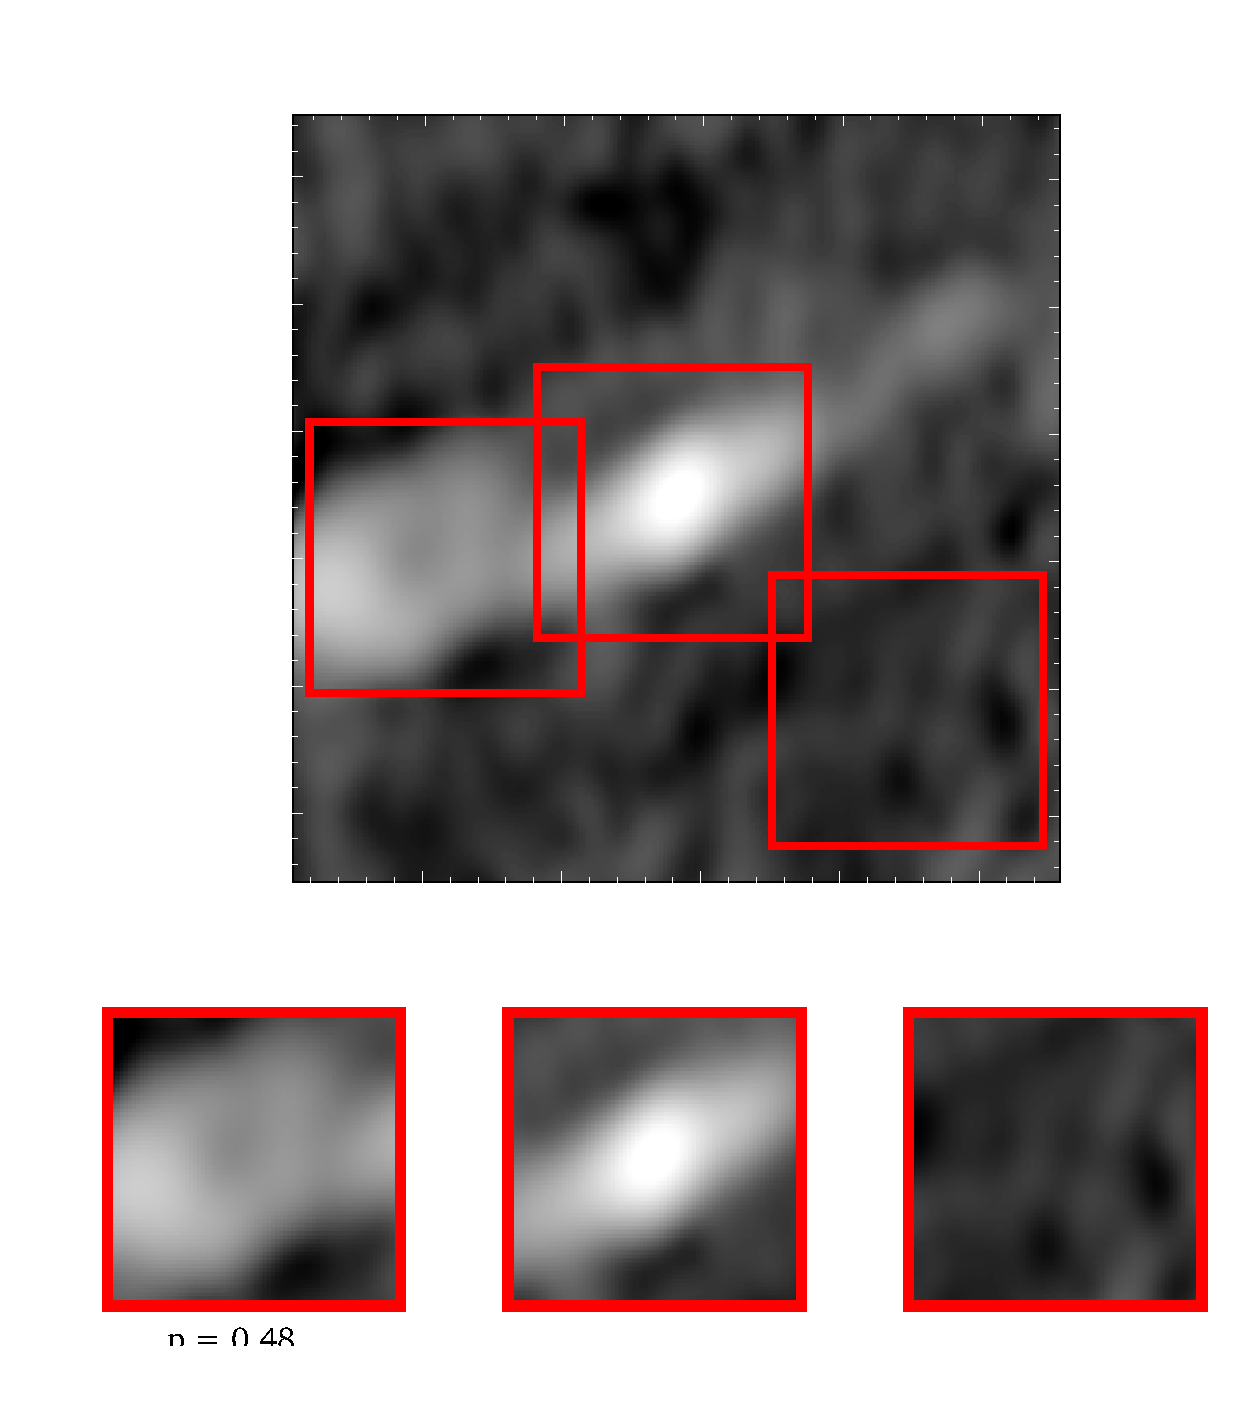
\includegraphics[width=\columnwidth]{images/elais_0093C1_with_boxes}
      \caption{An example of localising the host galaxy of a radio source using
        our method. This image is from ATLAS and is centred on $\alpha =
        00^\text{h}33^\text{m}06.36^\text{s}, \delta = -43^\circ{}10'30.1''$.
        Boxes represent $32 \times 32$ pixel windows centred on various
        locations in the image. The corresponding image patches from each
        window are shown beneath. The image patch of each window represents
        the location the window is centred on. The probabilities of each patch
        coinciding with the host galaxy would then be estimated by a
        classification model. The probabilities shown are for illustration
        only. In this example, the centre window of the image would be chosen
        as the location of the host galaxy, as the window centred on it has
        the highest probability.}
      \label{fig:windows}
    \end{figure}

  \subsection{Cross-identification as binary
  classification}\label{cross-identification-as-binary-classification}
    \begin{figure}
      \centering
      % http://www.texample.net/tikz/examples/simple-flow-chart/
      \tikzstyle{decision} = [diamond, draw, fill=white,
          text width=4.5em, text badly centered, inner sep=0pt]
      \tikzstyle{block} = [rectangle, draw, fill=white,
          text width=5em, text centered, rounded corners, minimum height=4em]
      \tikzstyle{line} = [draw, -latex']
      \begin{tikzpicture}[node distance=6mm, auto]
        \node [block] (init) {input radio source};
        \node [decision, right= of init] (iscompact) {compact?};
        \node [block, below= of iscompact] (compact) {find nearest infrared object};
        \node [block, right= of iscompact] (resolved) {find nearby infrared objects};
        \node [block, fill=black!10, right= of resolved] (classify) {classify objects};
        \node [block, below= of classify] (best) {find highest probability object};
        \coordinate (middle) at ($(compact)!0.5!(best)$);
        \node [block, below= of middle, fill=green!10] (done) {\textbf{host galaxy}};
        \path [line] (init) -- (iscompact);
        \path [line] (iscompact) -- (compact) node [midway] {yes};
        \path [line] (compact) -- (done);
        \path [line] (iscompact) -- (resolved) node [midway] {no};
        \path [line] (resolved) -- (classify);
        \path [line] (classify) -- (best);
        \path [line] (best) -- (done);
      \end{tikzpicture}
      \caption{A cross-identification method employing a binary classifier. As
        input we accept a radio source. If the source is compact, we select
        the nearest infrared object as the host galaxy. If the source is
        resolved, we classify all infrared objects nearby within radius $R$
        and select the highest probability object as the host galaxy. The grey
        box is the classifier, which can be any binary classifier that outputs
        a probability.}
      \label{fig:flowchart}
    \end{figure}

    We focus on the problem of host galaxy cross-identification without
    reference to radio morphology. Given a radio component, we want to find
    the corresponding host galaxy as a citizen scientist would using Radio
    Galaxy Zoo. The input is thus a radio image and an infrared image with a
    given radius. We choose a radius of 1~arcmin to match the size of the
    images used by Radio Galaxy Zoo. We make the assumption that each radio
    image represents a single, complex extended source. This is not the case
    in general and a radio image may contain many different radio sources with
    unique host galaxies. If we had access to radio morphology information, we
    could use this to isolate relevant components and hence more accurately
    cross-identify sources, but this is beyond the scope of this paper. We
    also note that this assumption will bias our results against radio
    emission that extends beyond the 1~arcmin cutout size, however, these are
    uncommon in ATLAS with 9 radio sources identified by \citet{norris06} as
    having components further than 1~arcmin apart (and of these, only 5 are in
    Radio Galaxy Zoo). The radio cross-identification task then amounts to
    locating the host galaxy within the associated radio and infrared images.
    This is formalised as an object localisation problem: given a radio image
    and an infrared image centred on a radio component, locate the host galaxy
    of the radio component.    % S031, S336, S081, S576, S136, S719, S618, S707, S287
    % ARG0003r2r, -, -, ARG0003r5h, ARG0003r2d, -, ARG0003r1s, -, ARG0003r8q

    A common approach to object localisation is to estimate the probability
    that each location in the image is coincident with the desired object. In
    practice this amounts to taking fixed-size windows of the image centred on
    each pixel and estimating the probability that each window is centred on
    the object. The location associated with the highest probability window is
    then assumed to be the location of the object. Applying this to radio host
    cross-identification, we consider windows of a radio/infrared image and
    estimate the probability that each window is centred on the host galaxy.
    This approach is illustrated in \autoref{fig:windows}. In computer vision
    a sliding window is commonly used: every possible patch in the image is
    considered \citep[e.g.][]{rowley1996facedetection}.

    This task can be made more efficient if we have a prior on the location of
    the object we are localising. For our prior, we assume that the host galaxy
    is always visible in the infrared and thus we only need consider windows
    centred on infrared sources. This assumption usually holds, except for a
    rare class of infrared-faint radio sources. \citet{norris06} found 22 such
    radio sources in their sample of 784 bright ATLAS components in CDFS. This
    leads us to a binary classification task: given an infrared source, compute
    the probability that it is a host galaxy. To find the host galaxy given a
    radio source, classify each galaxy within 1~arcmin of the source and select
    the galaxy with the highest probability of being a host galaxy. This is a
    good formulation as binary classification is a very common problem in
    machine learning and there are many different methods readily available to
    solve it.

    Solving the radio cross-identification task amounts to modelling a function
    $f$ from infrared sources $\mathcal{X}$ to the probability that an infrared
    source belongs to a binary class in $\mathcal{Y} = \{0, 1\}$:
    \begin{equation}
        f(x) \coloneqq \text{Pr}\left(\mathcal{Y} = 1 \mid \mathcal X = x\right)\,\,\,\,.
    \end{equation}
    The space of infrared sources $\mathcal{X}$ needs to be encoded as a vector
    for the models we will use. We describe this in
    \autoref{vector-representation-of-infrared-sources}. There are many options
    for modelling $f$. In this paper we apply three different models: logistic
    regression, random forests, and convolutional neural networks.

    We can improve upon this cross-identification method by filtering out
    compact radio sources, which are much easier to cross-identify --- the
    nearest SWIRE object may be identified as the host galaxy, or a more
    complex method such as likelihood ratios may be applied
    \citep[see][]{weston17}. A full cross-identification pipeline making use
    of this alongside a binary classifier is shown in \autoref{fig:flowchart}.

  \subsection{Limitations of our approach}
    \label{sec:limitations}

     \begin{figure}
      \centering
      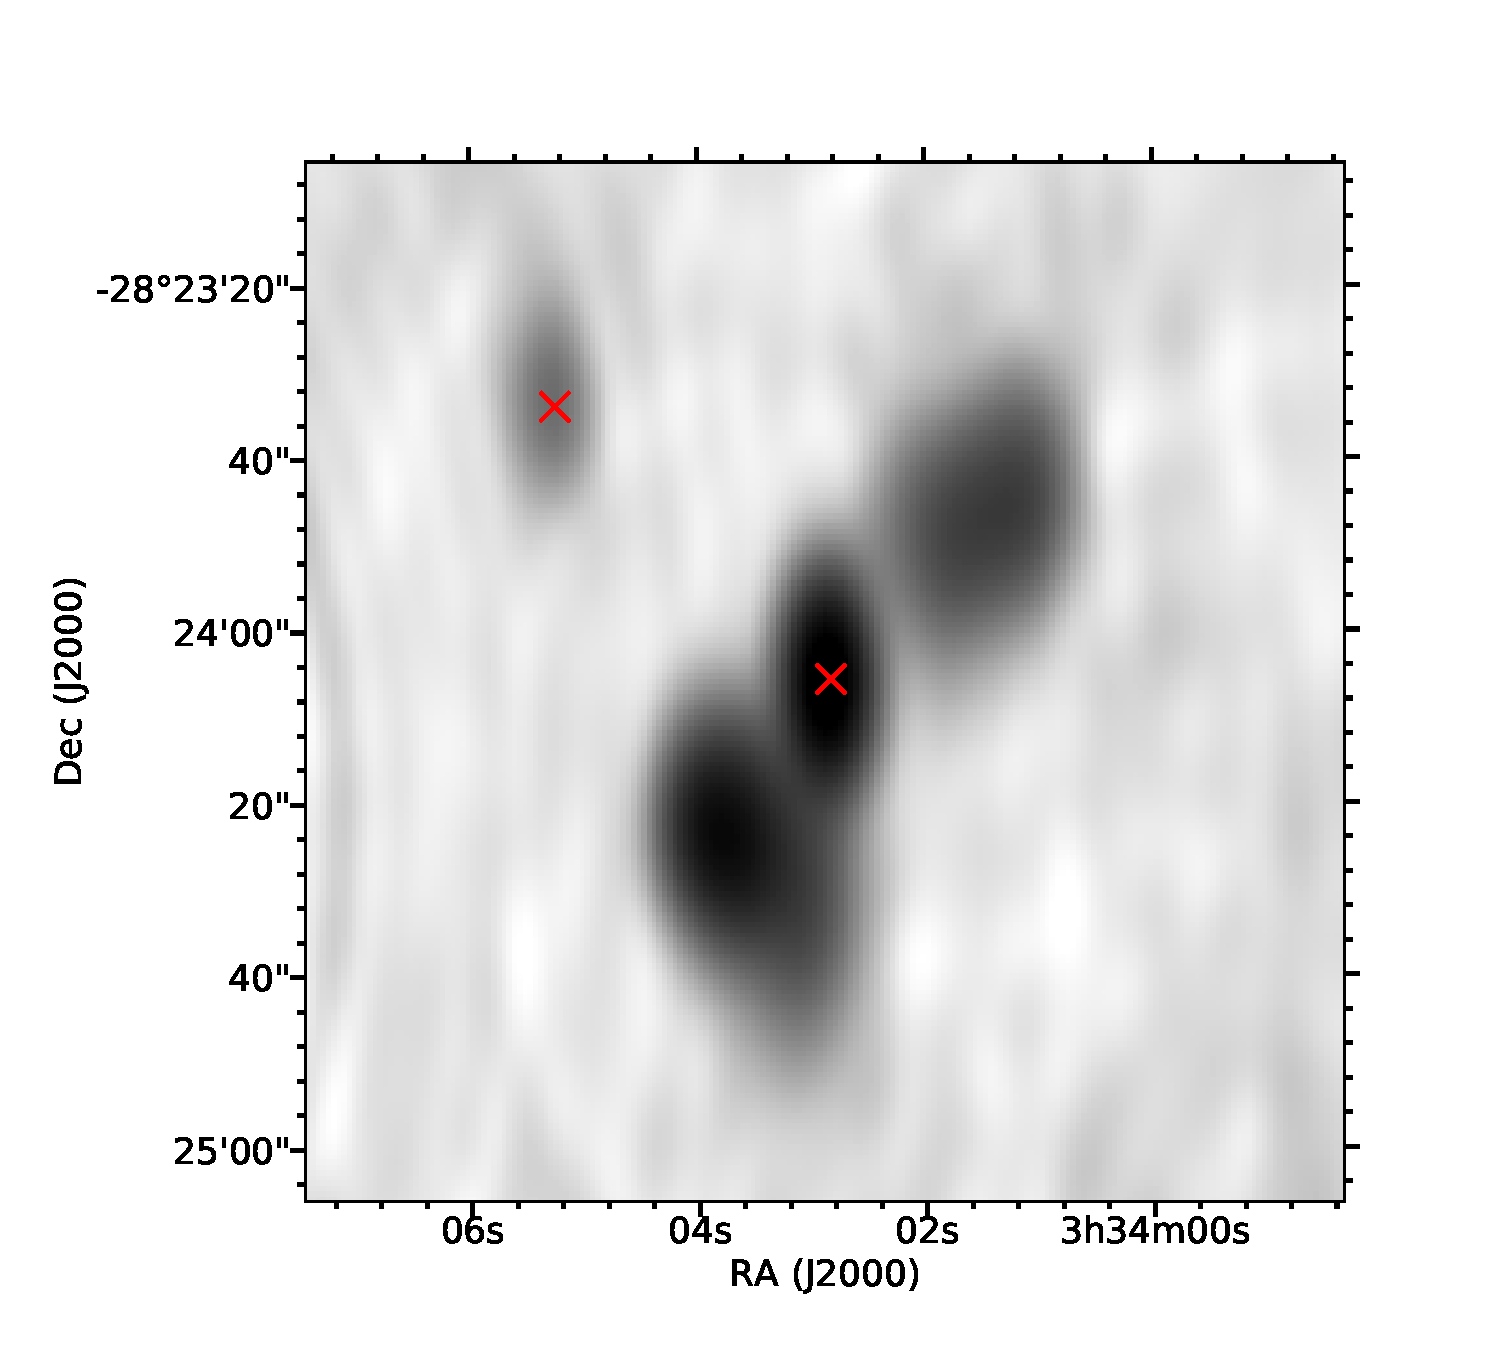
\includegraphics[width=\linewidth]{images/CI0077C1_fig.pdf}
      \caption{$2'$-wide radio image centred on ATLAS3\textunderscore{}J033402.87-282405.8C.
        %(ARG0003r2v)
        This radio source breaks our assumption that there are no other radio
        sources within 1~arcmin of the source. Another radio source is visible
        to the upper-left. Host galaxies found by Radio Galaxy Zoo volunteers
        are shown by a cross.}
      \label{fig:broken-isolation}
    \end{figure}

      \begin{figure}
      \centering
      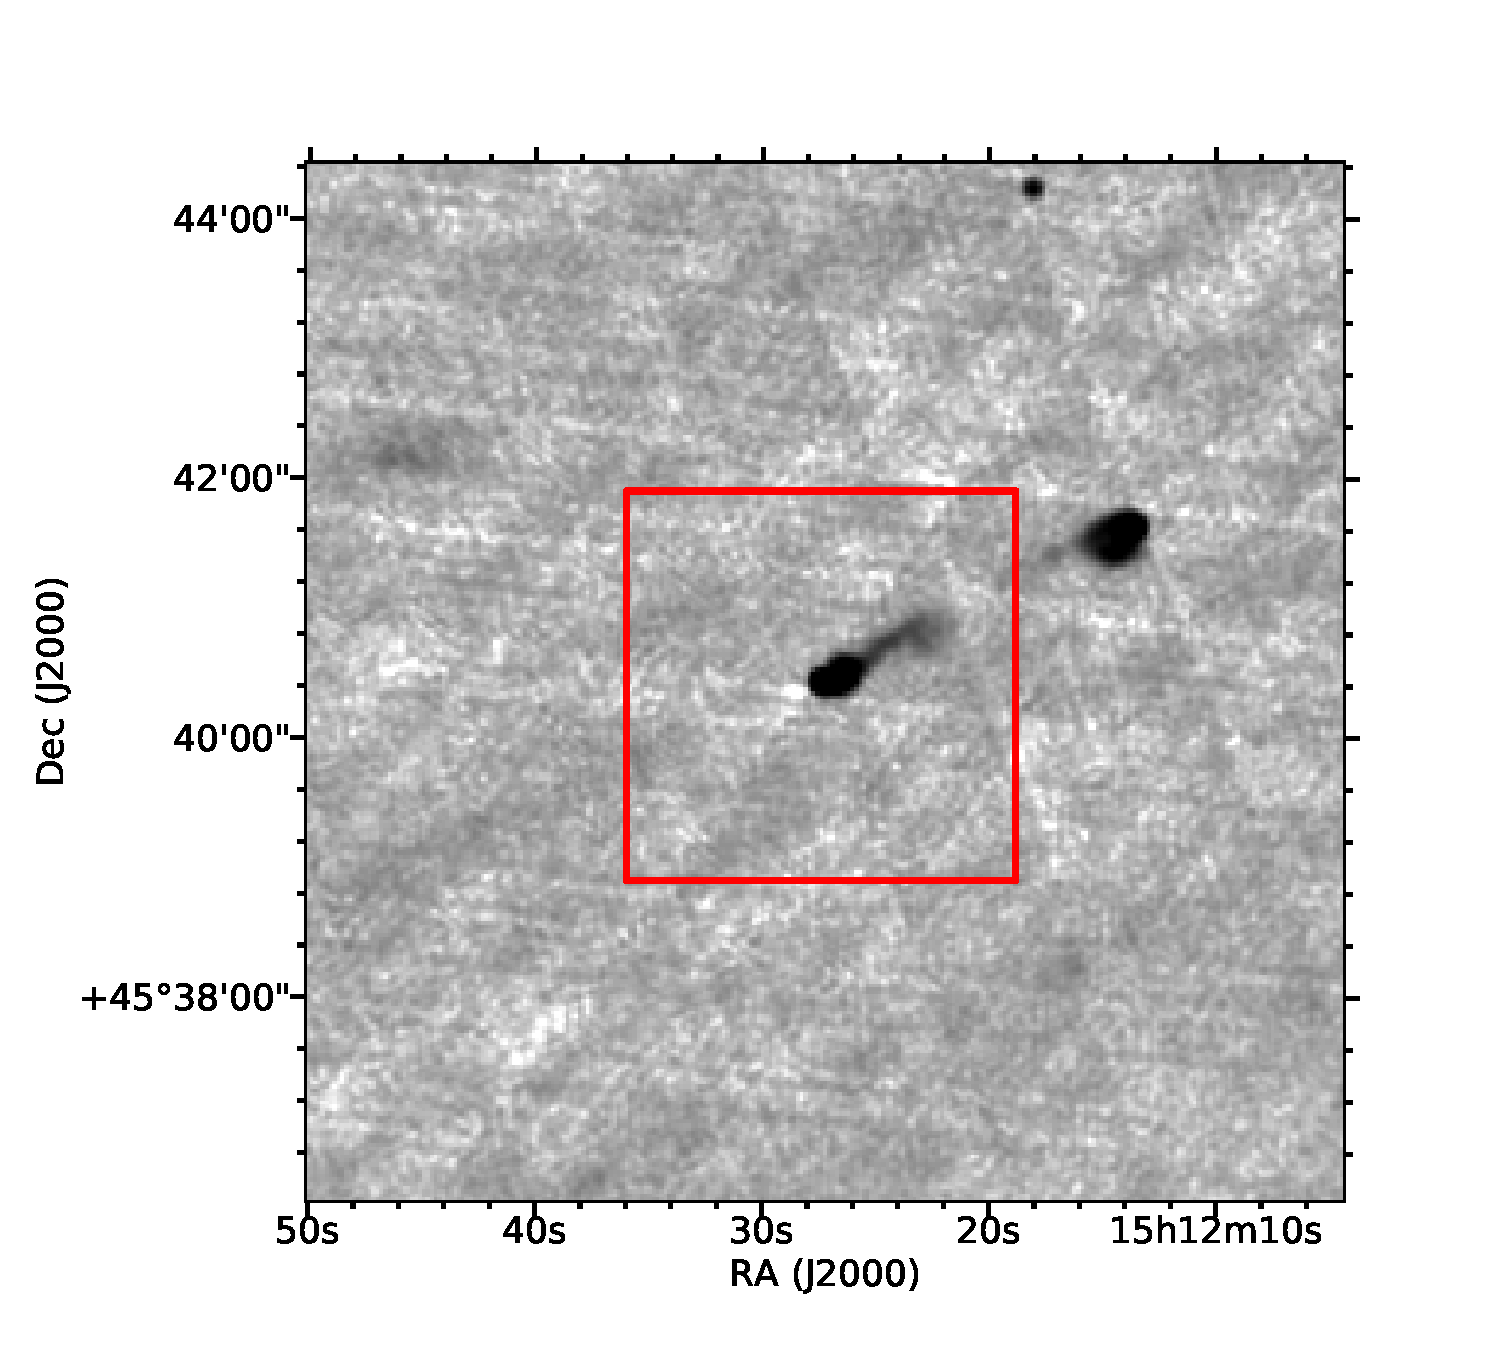
\includegraphics[width=\linewidth]{images/FIRSTJ151227_fig.pdf}
      \caption{A $8'$-wide radio image from FIRST, centred on
        FIRSTJ151227.2+454026. The $3'$-wide red box indicates the boundaries of
        the image of this radio component shown to volunteers in Radio Galaxy
        Zoo. This radio source breaks our assumption that the whole radio source
        is visible in the chosen radius. As one of the lobes of the radio source
        is outside of the image, a volunteer (or automated algorithm) looking at
        the $3'$-wide image may be unable to determine that this is a radio
        double or locate the host galaxy.}
      \label{fig:broken-contains}
    \end{figure}
        \begin{figure}
      \centering
      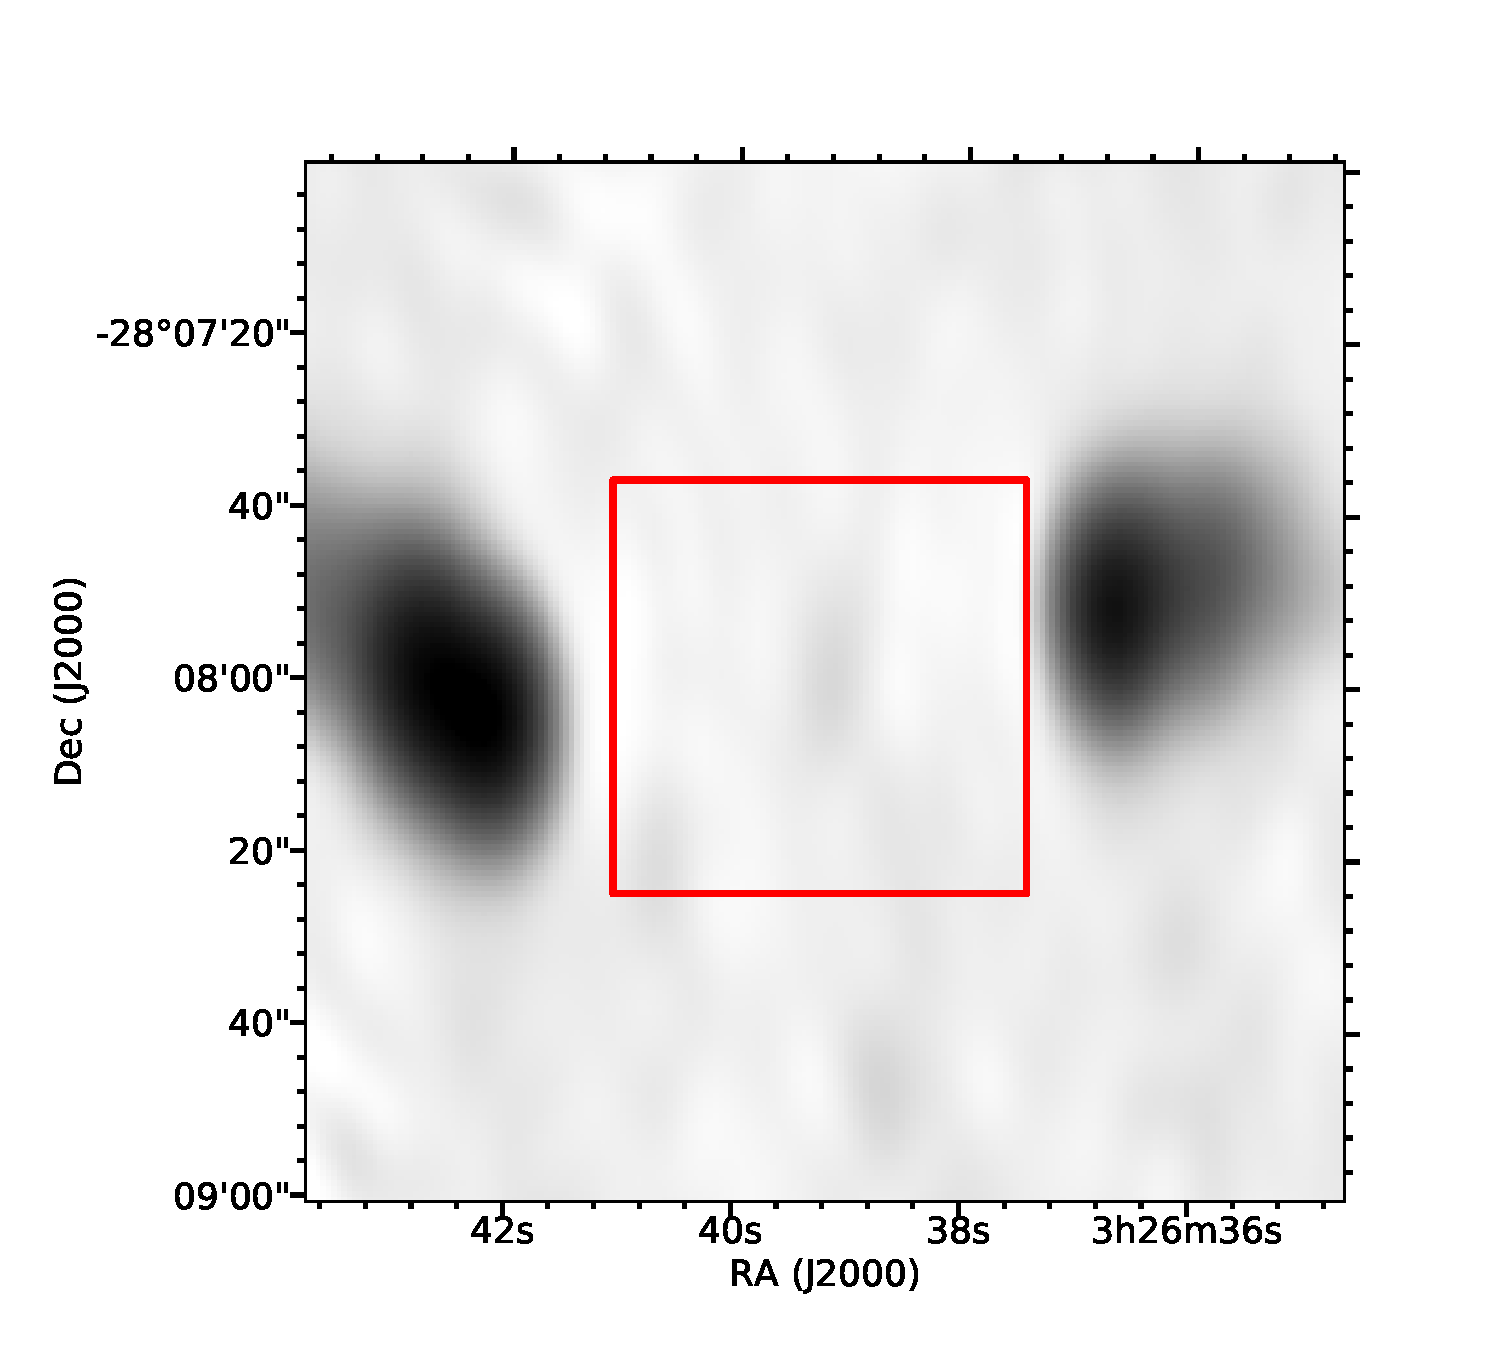
\includegraphics[width=\linewidth]{images/CI2363_fig.pdf}
      \caption{A radio image centred on $\alpha =
        03^\text{h}26^\text{m}39.12^\text{s}$, $\delta = -28^\circ{}07'58.80''$.        %ARG0003sky
        This is an example of a radio source where the window centred on the
        host galaxy, shown as a rectangle, does not contain enough radio
        information to correctly identify the galaxy as the host.}
      \label{fig:broken-window-size}
    \end{figure}

    We make a number of assumptions to reduce the cross-identification task to binary classification:
    \begin{itemize}
      \item A radio image represents a single radio source and contains exactly
        one host galaxy.
      \item The host galaxy of a radio component is within 1~arcmin of the
        component.
      \item The host galaxy appears in the SWIRE catalogue.
    \end{itemize}
    These assumptions limit the effectiveness of our approach, regardless of
    how accurate our binary classification may be.

    The key problem with this approach is our assumption that the radio sky
    within 1~arcmin radius contains only one, complete radio source. The problem
    is two-fold: This radius may contain multiple sources, or it may not contain
    the entirety of the source. If the radius contains multiple sources then
    there will also be multiple hosts in our input images (which breaks our
    assumption that there is only one); even a perfect classifier can only
    accurately cross-identify \emph{one} host in an image with multiple. An
    example of a radio source that breaks the assumption in this way is shown in
    \autoref{fig:broken-isolation}. If the radius does not contain the whole
    source, then we are missing radio information useful for finding the host
    galaxy. This is a difficult problem even for non-automated methods as radio
    sources can be extremely wide --- for example, Radio Galaxy Zoo found a
    radio giant that spanned over three different images presented to volunteers
    and the full source was only cross-identified by the efforts of citizen
    scientists \citep{banfield15}. An example of a radio image where part of the
    radio source is outside the search radius is shown in
    \autoref{fig:broken-contains}. The problems are in opposition to each other:
    To reduce the number of sources in an input image, we can reduce the image
    radius, but this increases the chance that we will miss relevant radio
    source information, and vice versa.

    Our assumptions impose an upper bound on how well we can cross-identify
    radio sources, which can be estimated by considering how accurately a
    \emph{perfect} binary classifier cross-identifies radio sources under our
    method. Using the expert labels (\autoref{labels}) to classify SWIRE objects
    to 100~percent accuracy on the binary classification task results in a
    cross-identification accuracy of $(96.74 \pm 1.76)$~percent across the four
    CDFS quadrants under our assumptions, which we take as an upper bound on our
    cross-identification accuracy.

    A related issue is that we need to choose a window size for the image
    representations of each SWIRE object. If this image is too small, radio
    emission may extend past the edges of the window, and it may be impossible
    to identify the galaxy as a host galaxy. If the image is too large, then
    too much information will be included and it will be difficult or
    computationally expensive to classify. We chose a window size of $32
    \times 32$ pixels, shown as a red rectangle in
    \autoref{fig:windows} and \autoref{fig:broken-window-size}.

  \subsection{Feature vector representation of infrared sources}
  \label{vector-representation-of-infrared-sources}

    Binary classification methods require that the inputs to be classified are
    represented by an array of real values called \emph{feature vectors}. We
    thus need to choose a feature vector representation of our candidate host
    galaxies.

    Infrared observations of the CDFS field are taken from SWIRE. We use the
    CDFS Fall '05 SWIRE catalogue \citep{surace05swire} to generate candidate
    hosts to classify. Radio observations of the CDFS field are taken from
    ATLAS. The radio image is taken to be a 32 $\times$ 32 pixel image from
    ATLAS, centered on the candidate host location from SWIRE.
    As the visual appearance of objects in SWIRE are likely irrelevant to
    whether the galaxy is a host galaxy, the candidate host location encodes
    almost all information we could gain from the infrared image. We therefore
    do not use the infrared image for object localisation.

    We represent each candidate host as 1034 real-valued features. For a given
    candidate host, these features are:
    \begin{itemize}
      \item the logarithm of the ratio of fluxes of the candidate host in the
        four IRAC wavelengths;
      \item the stellarity index of the host in both 3.6 and
        \unit{4.5}{\micro\meter};
      \item the flux of the host in \unit{3.6}{\micro\meter};
      \item the radial distance between the candidate host and the nearest
        radio component in the ATLAS catalogue; and
      \item a 32 $\times$ 32 pixel image from ATLAS, centred on the candidate
        host.
    \end{itemize}

    The infrared fluxes provide insight into the properties of the host galaxy
    of the radio emission. The 3.6 and \unit{4.5}{\micro\meter} fluxes trace
    both galaxies with faint polycyclic aromatic hydrocarbon (PATH) emission and
    elliptical galaxies dominated by old stellar popluations. The
    \unit{5.8}{\micro\meter} flux selects galaxies where the infrared emission
    is dominated by non-equilibrium emission of dust grains (PAH destruction
    by the hard UV spectrum of AGN), while the \unit{8.0}{\micro\meter} flux
    traces strong PAH emission at low redshift \citep{Sajina2005}.
    The stellarity index represents how likely the object is to be a star
    rather than a galaxy.

    We use the pixels of each $32 \times 32$ radio image as
    independent features for all classifiers, with the convolutional neural
    network (Section \ref{sec:convolutional-neural-networks}) automatically
    extracting features that are relevant.
    There has been limited research on extracting features from radio images.
    \citet{proctor06} describe hand-selected features for radio doubles in
    FIRST, and \citet{aniyan17cnn} and \citet{lukic17compact} make use of deep
    convolutional neural networks which automatically extract features as part
    of classification. A more comprehensive search of neural network architectures
    for processing radio images is beyond the scope of this initial study,
    and is a good avenue for potential improvement in our pipeline.

  \subsection{Classifiers}\label{sec:classifiers}

    We use three different classifiers as our binary classification model:
    logistic regression, convolutional neural networks, and random forests.

    \subsubsection{Logistic Regression}
    \label{sec:logistic-regression}
      Logistic regression is a binary classification model. It is linear in the
      feature space and outputs the probability that the input has a positive
      label. The model is \citep{bishop06ml}:

      \begin{equation}
          f(\vec x) = \sigma(\vec w \cdot \vec x + b) \,\,\,\,,
      \end{equation}
      where $\vec w \in \mathbb{R}^D$ is a weights vector,
      $b \in \mathbb{R}$ is a bias term, $\vec x \in \mathbb{R}^D$ is the
      feature representation of a candidate host, and $\sigma$ is the
      logistic sigmoid function: \begin{equation}
          \sigma(a) = (1 + \mathrm{exp}(-a))^{-1}\,\,\,\,.
      \end{equation}%
      The logistic regression model is fully differentiable, and the weights
      vector $\vec w$ can therefore be learned using gradient methods.

    \subsubsection{Convolutional neural networks}
    \label{sec:convolutional-neural-networks}

      Convolutional neural networks (CNN) are a biologically-inspired prediction
      model for prediction with image inputs. A number of filters are convolved
      with an input image to produce output images called \emph{feature maps}.
      These feature maps can then be convolved again with other filters on
      subsequent layers, producing a network of convolutions. The whole network
      is differentiable with respect to the values of the filters and the
      filters can be learned using gradient methods. The final layer of the
      network is logistic regression, with the convolved outputs as input
      features. For more detail, see \citet[subsection II.A][]{lecun98}. We use
      \textsc{Keras} \citep{chollet15keras} to implement our CNN.

      % \begin{figure*}
      %   \centering
      %   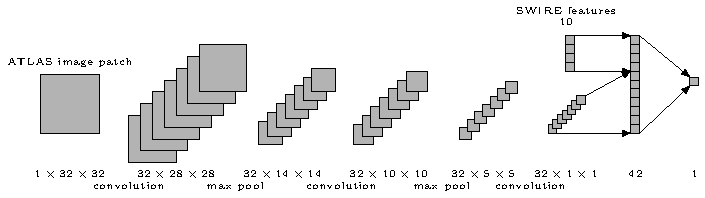
\includegraphics[width=\textwidth]{convnet.pdf}
      %   \caption{Convolutional neural network model.}
      %   \label{fig:cnn}
      % \end{figure*}

      \begin{figure}
        % \begin{tabular}{l|c}
        %   \hline
        %   Layer type & Output size\\
        %   \hline
        %   Image Input & $1 \times 32 \times 32$\\
        %   Convolution & $32 \times 28 \times 28$\\
        %   Max pooling & $32 \times 14 \times 14$\\
        %   Convolution & $32 \times 10 \times 10$\\
        %   Max pooling & $32 \times 5 \times 5$\\
        %   Dropout & $32 \times 5 \times 5$\\
        %   Merge & $810$\\
        %   Logistic regression & $1$\\
        %   \hline
        % \end{tabular}
        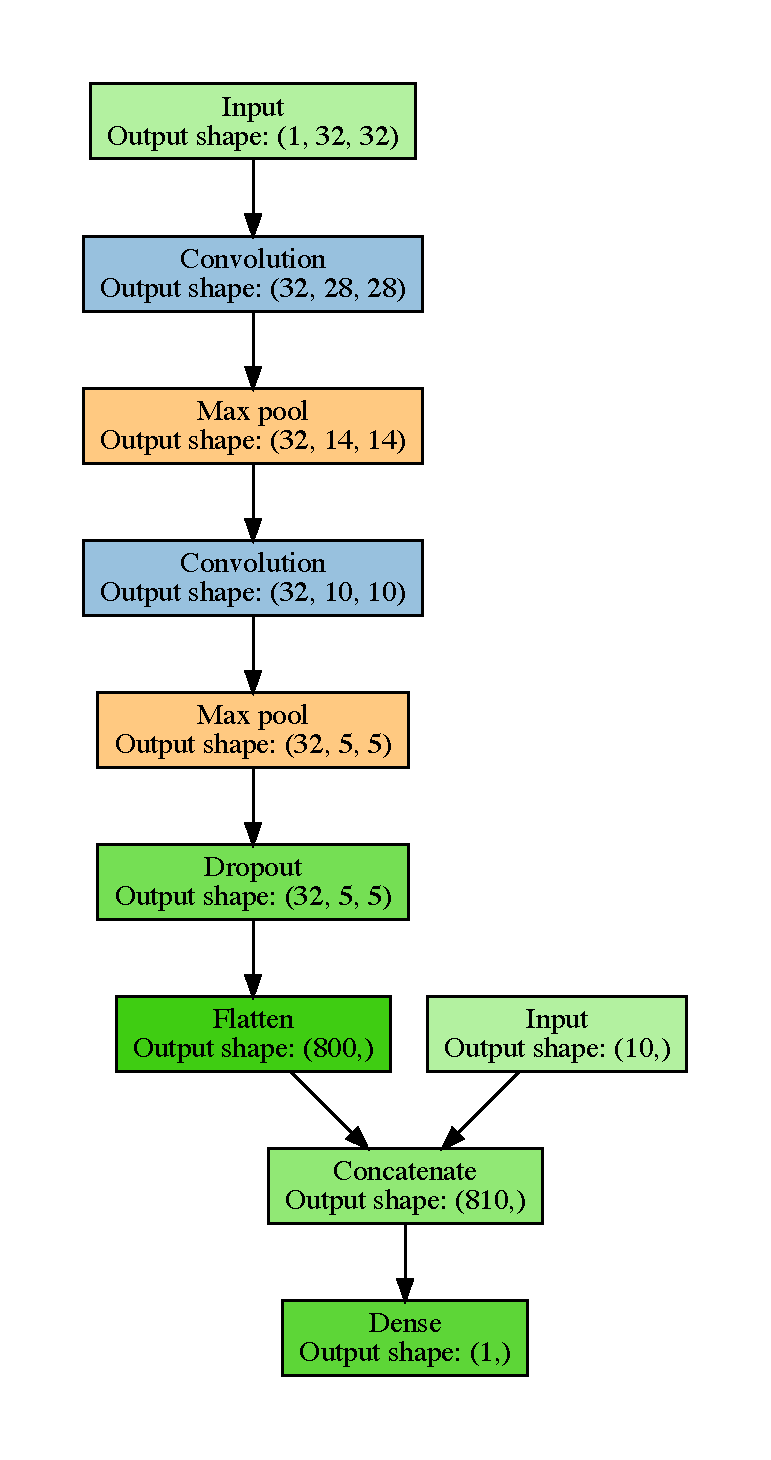
\includegraphics[width=\linewidth]{images/cnn_model_graph}
        \caption{Architecture of our CNN. The merge layer flattens the output of
          the previous layer and adds the 10 features derived from the
          candidate host in SWIRE, i.e. the flux ratios, stellarity indices,
          and distance. The dropout layer drops $25\%$ of its
          inputs. Diagram based on \url{
          https://github.com/dnouri/nolearn}.}
        \label{fig:cnn}
      \end{figure}

      CNNs have recently produced good results on large image-based datasets in
      astronomy \citep[e.g.][]{dieleman15cnn, lukic17compact}. We employ only a
      simple CNN model in this paper as a proof of concept that CNNs may be used
      for class probability prediction on radio images. The model architecture
      we use is shown in \autoref{fig:cnn}.

    \subsubsection{Random Forests}
    \label{sec:random-forests}

      Random forests are an ensemble of decision
      trees~\citep{breiman01random-forest}. It considers multiple subsamples
      of the training set, where each bootstrap subsample is sampled with
      replacement from the training set. For each subsample a decision tree
      classifier is constructed. The decision tree is built by repeatedly
      making axis-parallel splits based on individual features. In a random
      forest the split decision is taken based on a random subset of features.
      To classify a new data point, the random forest takes the weighted
      average of all classifications produced by each decision tree.

  \subsection{Labels}\label{sec:labels}
    \begin{figure}
      \centering
      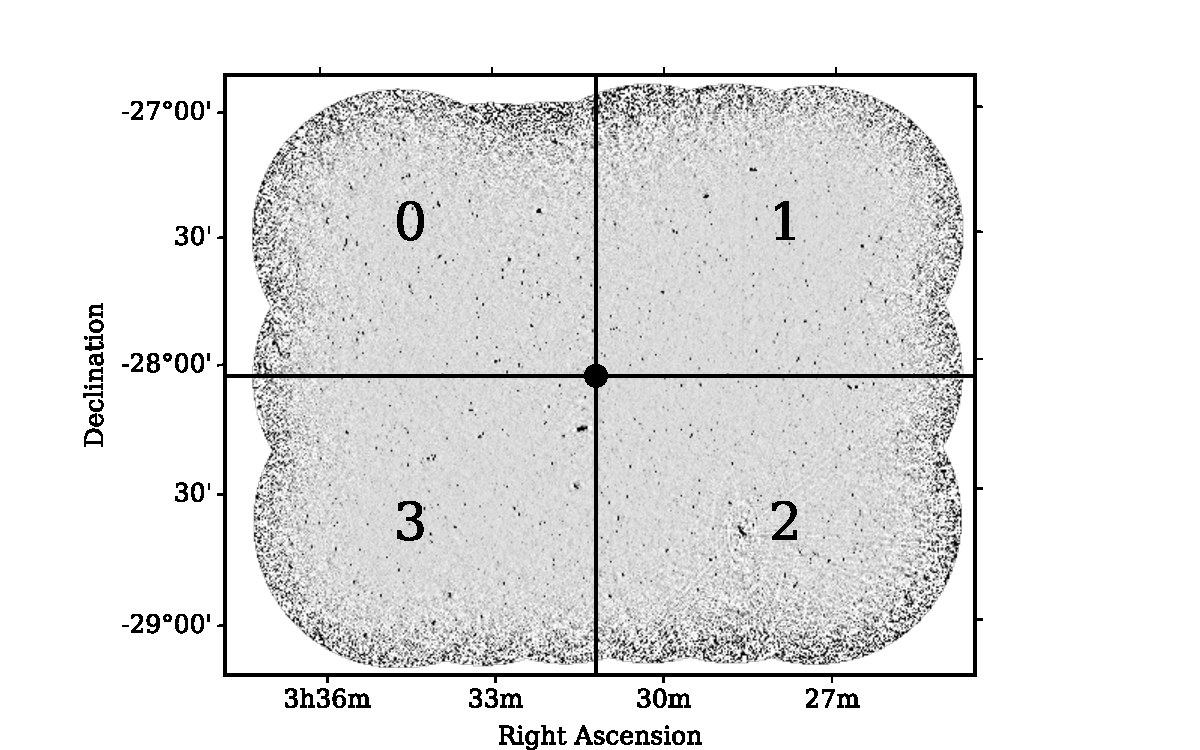
\includegraphics[width=\columnwidth]{images/quadrants.pdf}
      \caption{CDFS field training and testing quadrants labelled 0 -- 3. The
        central dot is located at $\alpha = 03^\text{h}31^\text{m}12^\text{s},
        \delta = -28^\circ{}06'00''$. The quadrants were chosen such that
        there are similar numbers of radio sources in each
        quadrant.\label{fig:quadrants}}
    \end{figure}

    \begin{figure}
      \centering
      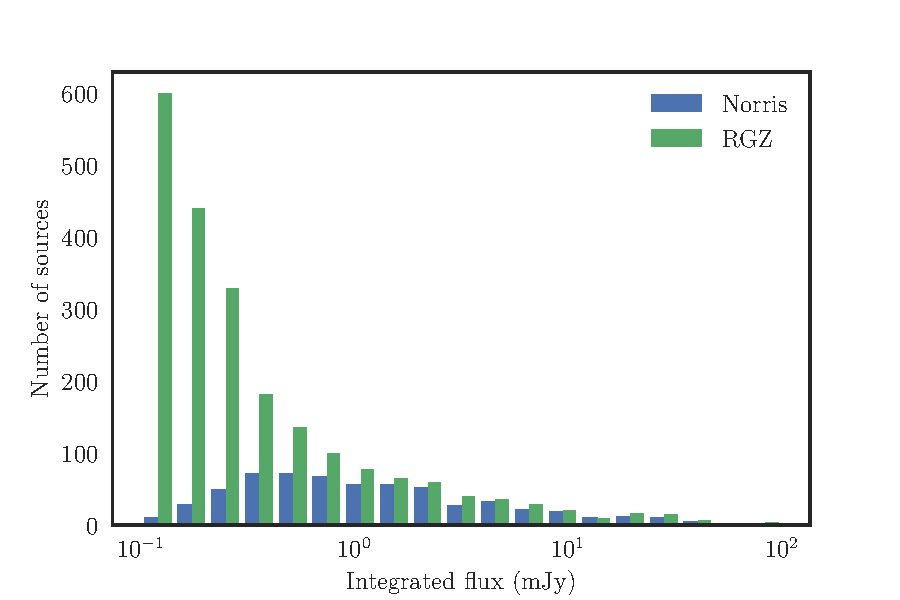
\includegraphics[width=\columnwidth]{images/flux_histogram.pdf}
      \caption{Distribution of integrated flux for radio components
        cross-identified in ATLAS DR1 (Norris) and by Radio Galaxy Zoo (RGZ).
        Radio Galaxy Zoo has cross-identified considerably more faint
        objects.}
      \label{fig:distribution-fluxes}
    \end{figure}

    \begin{figure}
      \centering
      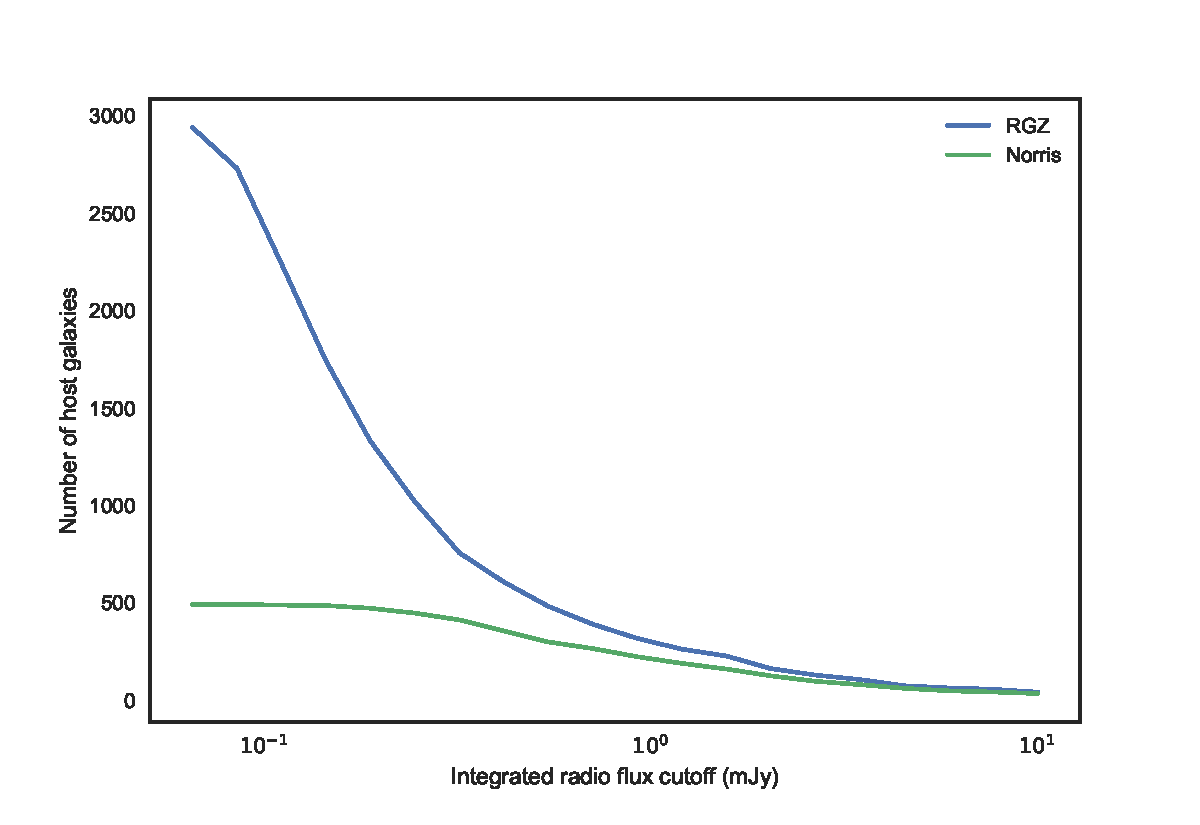
\includegraphics[width=\columnwidth]{images/host_galaxies_flux_cutoff.pdf}
      \caption{Number of host galaxies in the expert (Norris) and Radio Galaxy
        Zoo (RGZ) training sets with different integrated radio flux cutoffs.
        The two training sets converge to the same number of host galaxies as
        the cutoff is increased.}
      \label{fig:distribution-cutoffs}
    \end{figure}

    Converting the Radio Galaxy Zoo and \citet{norris06} cross-identification
    catalogues to binary labels for infrared objects is a non-trivial task. A
    clear problem is that there is no way to capture radio morphology
    information in binary classification. As a result, we ignore this problem
    for this paper. Another problem is that there is no way to indicate
    \emph{which} radio object an infrared object is associated with, only that
    it is associated with \emph{some} radio object. We make the na\"ive
    assumption that any given radio image contains only one host galaxy as the
    first step in solving this problem.

    We then generate positive labels from a cross-identification catalogue.
    We decide that if an infrared object is listed in the catalogue, then it
    is assigned a positive label as a host galaxy. In principle we would
    then assign every other galaxy a negative label. This has some problems
    --- an example is that if the cross-identifier did not observe a radio
    object (e.g.~it was below the signal-to-noise ratio) then the host galaxy
    of that radio object would receive a negative label. This occurs with
    \citet{norris06} cross-identifications, as these are associated with the
    first data release of ATLAS. The first data release went to a 5$\sigma$
    flux density level of $S_{1.4} \geq 1 \text{ mJy beam}^{-1}$
    \citep{norris06}, compared to $S_{1.4} \geq \unit{85}{\micro\jansky}\text{
    beam}^{-1}$ for the third data release used by Radio Galaxy Zoo
    \citep{franzen15}. The expert labels may therefore disagree with labels
    from Radio Galaxy Zoo even if they are both plausible. The difference in
    flux distributions between the expert and Radio Galaxy Zoo
    cross-identified sources is shown in \autoref{fig:distribution-fluxes} and
    the difference in training set size at different flux cutoffs is shown in
    \autoref{fig:distribution-cutoffs}. We train and test our classifiers on
    infrared objects within a 1~arcmin radius of an ATLAS radio object.

  \subsection{Experimental Setup}
  \label{sec:experimental-setup}

    We trained cross-identifiers on radio objects from the ATLAS observations of
    the CDFS field, using two label sets. One label set was derived from Radio
    Galaxy Zoo cross-identifications and the other was derived from the
    \citet{norris06} cross-identification catalogue. We refer to these as the
    Radio Galaxy Zoo labels and the expert labels respectively. We divided the
    CDFS field into four quadrants for training and testing. The quadrants were
    centred on $\alpha = 52^\text{h}48^\text{m}00^\text{s},
    \delta = -28^\circ{}06'00''$ as shown in \autoref{fig:quadrants}. For
    each trial, one quadrant was used to draw test examples and the other three
    quadrants were used for training examples.

    We further divided the radio components into compact and resolved. Compact
    components are cross-identified by fitting a 2D Gaussian \citep[as
    in][]{norris06} and we would expect any machine learning approach for host
    cross-identification to attain high accuracy on this set. Whether a
    component was resolved was decided based on its flux; a radio component was
    considered resolved if
    \begin{equation}
        \ln \left(
          \frac{S_{\text{int}}}
               {S_{\text{peak}}}
        \right) > 2\sqrt{\left(
          \frac{\sigma_{S_{\text{int}}}}
               {S_{\text{int}}}
        \right)^2 + \left(
          \frac{\sigma_{S_{\text{peak}}}}
               {S_{\text{peak}}}
        \right)^2}\,\,\,\,,
    \end{equation}%
    where \(S_{\text{int}}\) is the integrated flux density and
    \(S_{\text{peak}}\) is the peak flux density \citep{franzen15}.

    Candidate hosts were selected from the SWIRE catalogue. For a given subset
    of radio components, all SWIRE objects within 1~arcmin of all radio
    components in the subset were added to the associated SWIRE subset. In the
    context of the binary classification task, we refer to SWIRE objects
    within 1~arcmin of a compact radio component as part of the `compact set',
    and SWIRE objects within 1~arcmin of a resolved radio component as part of
    the `resolved set'.

    Classifiers were trained on all available training data in the training
    quadrants. Test examples were drawn from the remaining quadrant. To reduce
    bias in the testing data due to the expert labels being generated from a
    shallower data release of ATLAS, a SWIRE object was only added to the test
    set if it was within 1~arcmin of a radio object with a cross-identification
    in both the \citet{norris06} catalogue and the Radio Galaxy Zoo catalogue.

    Each classifier was trained on the training examples and used to predict
    labels for the test examples. The predicted labels were compared to the
    expert labels and the balanced accuracy was computed. We use balanced
    accuracy as our accuracy measure due to the highly imbalanced classes --- in
    our total set of SWIRE objects within 1~arcmin of an ATLAS object, only
    4~percent have positive labels. Only examples within 1~arcmin of ATLAS
    objects in the first ATLAS data release \citep{norris06} were used to
    compute accuracy, as these were the only ATLAS objects with expert labels.

    We then used the outputs of our classifiers to predict the host galaxy for
    each radio component cross-identified by both \citet{norris06} and Radio
    Galaxy Zoo. For each SWIRE object within 1~arcmin of the radio component,
    the probability of the object having a positive label was estimated using
    the trained binary classifiers. The SWIRE object with the highest
    probability was chosen as the host galaxy. The accuracy was then estimated
    by counting how many predicted host galaxies matched the \citet{norris06}
    cross-identifications.

\section{Results}\label{sec:results}

  \cheng{Describe the section}

  \subsection{Relation between binary classification and cross-identification}

  We report two sets of accuracies: first, the balanced accuracies for the
  task of classifying individual SWIRE objects as host galaxies or not host
  galaxies (the `galaxy classification task'); and second, the accuracies
  for the task of cross-identifying ATLAS radio components with their host
  galaxies (the `cross-identification task'). Balanced accuracy is a useful
  metric for evaluating classifiers on classification tasks with highly
  imbalanced classes like we have here, and we find that the balanced
  accuracy on the galaxy classification task is correlated with the accuracy
  on the cross-identification task for logistic regression classifiers. This
  correlation is shown in \autoref{fig:gct-to-xid}.

  \cheng{Describe upper and lower bounds}

  \subsection{Application to ATLAS-CDFS}

    \begin{figure}
      \centering
      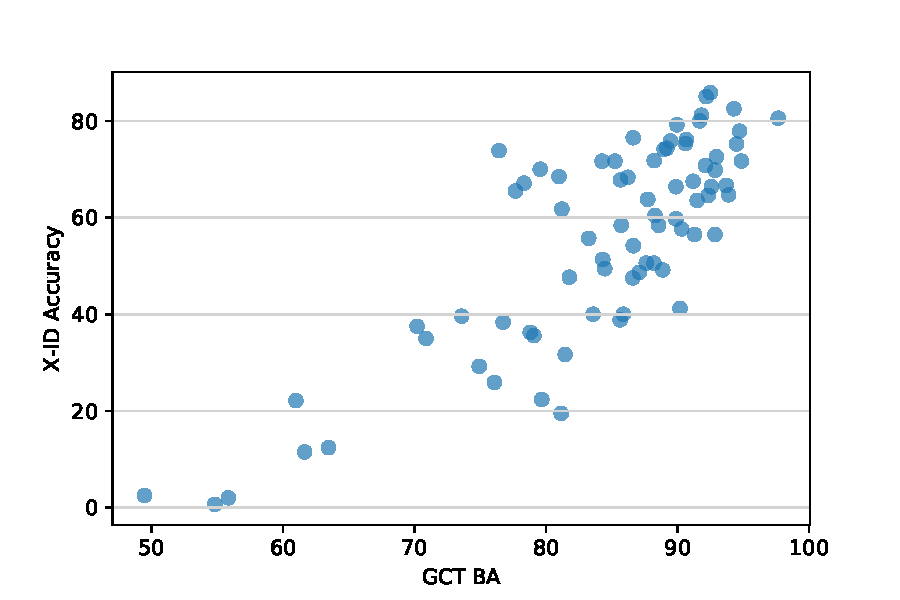
\includegraphics[width=\columnwidth]{gct-to-xid.pdf}
      \caption{Balanced accuracy on the galaxy classification task (GCT) plotted
      against accuracy on the cross-identification task (X-ID). RF indicates
      results from random forests, and LR indicates results from logistic
      regression. Classifiers were trained on random, small subsets of the
      training data to artificially restrict their accuracies. Colour shows
      the density of points on the plot estimated by a Gaussian kernel density
      estimate. The high density of points at 50 per cent balanced accuracy, 0
      per cent cross-identification accuracy for random forests is an artefact
      of our method of classifier generation, as random forests have much
      lower performance than logistic regression with less training data.
      \label{fig:gct-to-xid}}
    \end{figure}

    \begin{figure}
    \centering
    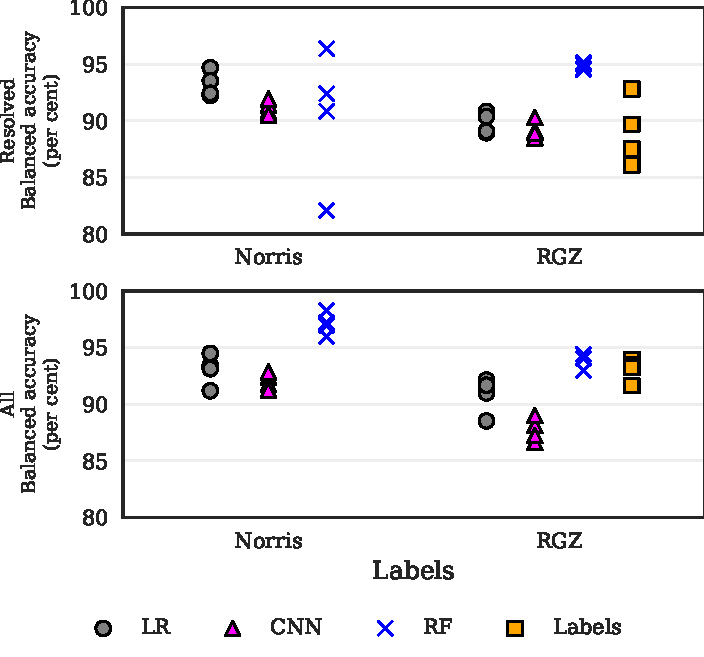
\includegraphics[width=\columnwidth]{images/cdfs_ba_grid.pdf}
    \caption{Balanced accuracies for each quadrant in the galaxy
      classification task. The accuracies of different classifiers are represented
      by different shapes. The horizontal axis shows which label set was used to
      train the classifiers: `Norris' represents the expert labels, `RGZ'
      represents the Radio Galaxy Zoo labels.
      %, and `RGZ N' represents the Radio
      %Galaxy Zoo labels applied only to the radio components that appeared in the
      %expert cross-identification catalogue.
      The three plots show different sets
      of training and testing data: the `compact' contains only compact radio
      components, `resolved' only contains resolved radio components, and `all'
      contains all radio components.
      %The maximum attainable balanced accuracy is
      %100~percent, when every galaxy label matches the expert labels.
      \label{fig:ba}}
    \end{figure}

    \begin{figure}
      \centering
      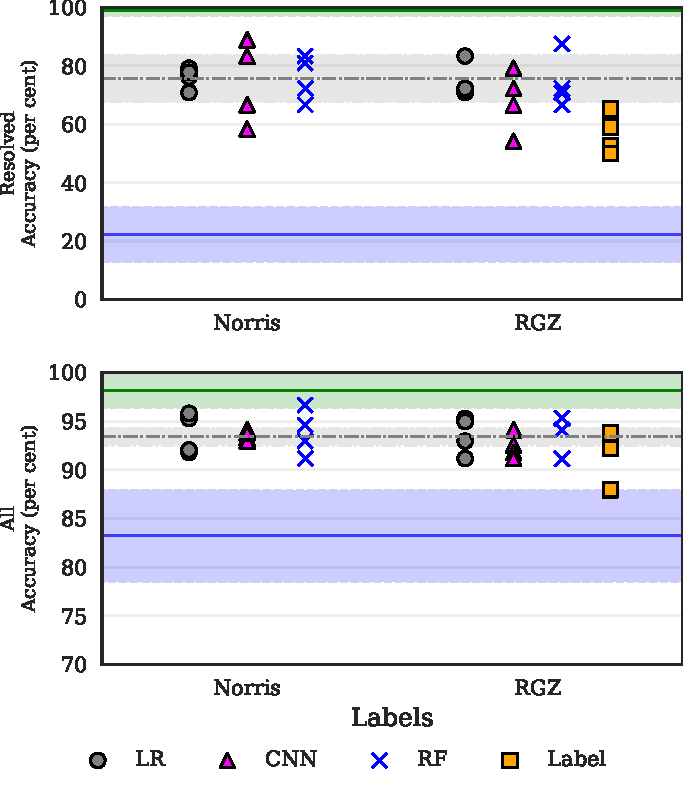
\includegraphics[width=\columnwidth]{images/cdfs_cross_identification_grid.pdf}
      \caption{Accuracies for each quadrant in the cross-identification
        task. Markers and axes are as in \autoref{fig:ba}. The upper horizontal line
        indicates the accuracy of a `perfect' classifier on the cross-identification
        task, with the surrounding dashed lines indicating the standard deviation
        across CDFS quadrants. A `perfect' classifier simply reads the expert
        labels. This represents the maximum attainable cross-identification accuracy
        under our assumptions. The lower horizontal line indicates the average
        accuracy of 15 random classifiers, and hence represents the minimum accuracy
        we would expect to attain. The surrounding dashed lines indicate the
        standard deviation across CDFS quadrants and classifiers.
        \label{fig:cross-id-accuracy}}
    \end{figure}

    For the galaxy classification task, we report the balanced accuracy of
    each classification model and training set in \autoref{fig:ba} for SWIRE
    objects within 1~arcmin of (1) compact radio components, (2) resolved
    radio components, and (3) all radio components. These accuracies averaged
    across the four quadrants are reported in
    \autoref{tab:average-accuracies}. We find that the classifiers trained on
    expert labels generally outperform \cheng{This is a tough claim} those trained on Radio Galaxy Zoo
    labels on almost all classification models, with random forests trained
    and tested on the resolved set as the only exception. This is likely due
    to the very small size of the expert-labelled resolved set, which had only
    labelled 98 host galaxies across CDFS compared to 150 host galaxies for
    the Radio Galaxy Zoo-labelled set. This is supported by the high spread of
    balanced accuracies for random forests trained on the expert-labelled
    resolved set, which have a standard deviation of $4.8$ percentage points
    compared to a standard deviation of $0.6$ percentage points when trained
    on the Radio Galaxy Zoo-labelled resolved set. Despite being lower, the
    accuracies attained by the classifiers trained on Radio Galaxy Zoo labels
    are still comparable to those trained on expert labels, with most Radio
    Galaxy Zoo-trained models achieving accuracies within a few percentage
    points of the expert-trained models.
    \cheng{Discuss separately: difference between methods (LR, CNN, RF),
    difference between labellers (Norris, RGZ).}

    We report the probabilities predicted by each classifier for each SWIRE
    object in \autoref{tab:probs}. Probabilities reported for a given object
    were predicted by classifiers tested on the quadrant containing that
    object.

    For the cross-identification task, we report the accuracy of each
    classification model and training label set in
    \autoref{fig:cross-id-accuracy}. We report the averaged
    cross-identification accuracies across all four quadrants in
    \autoref{tab:cross-id-accuracies}. Logistic regression produces the most
    consistent performance across label sets, with very little variation in
    accuracy between expert-trained and Radio Galaxy Zoo-trained logistic
    regression. Random forests perform well when trained on expert labels,
    but, unlike in the galaxy classification task, perform poorly when trained
    on Radio Galaxy Zoo labels. The high spread of accuracies associated with
    expert-trained random forests in the galaxy classification task is not
    reflected in the accuracies of the cross-identification task.
    Convolutional neural networks outperform the other expert-trained methods
    on the dataset containing all sources, in contrast to their relatively low
    performance on the galaxy classification task.

    The predicted cross-identification for each ATLAS object is reported in
    \autoref{tab:cids}. As with SWIRE predicted probabilities, reported
    cross-identifications for a given object were generated by classifiers
    tested on the quadrant containing that object.

    In \autoref{fig:cnnexamples} we show examples of where the incorrect
    cross-identification was selected by the CNN trained on expert labels. We
    find that radio components with multiple possible SWIRE host galaxies,
    radio images with multiple radio sources, and radio images with radio
    components extending beyond the edge of the image are problematic for the
    classifier. We also note in (c), (d), and (h) that the classifier tends to
    mistake radio lobes as core emission and thus assigns high probabilities
    to SWIRE objects near a lobe. This is likely due to the large number of
    compact objects in the training data --- at the resolution of ATLAS, most
    objects in CDFS appear compact (or very close to compact).

    We have noted in \autoref{sec:labels} that the test set of expert labels,
    derived from the initial ATLAS data release, was less deep than the third
    data release used by Radio Galaxy Zoo and this paper, introducing a source
    of label noise in the testing labels. Specifically, true host galaxies may
    be misidentified as non-host galaxies if the associated radio source was
    below the $5\sigma$ flux density limit in ATLAS DR1 but not in ATLAS DR3.
    This has the effect of reducing the accuracy for Radio Galaxy Zoo-trained
    classifiers.

  \begin{figure*}
  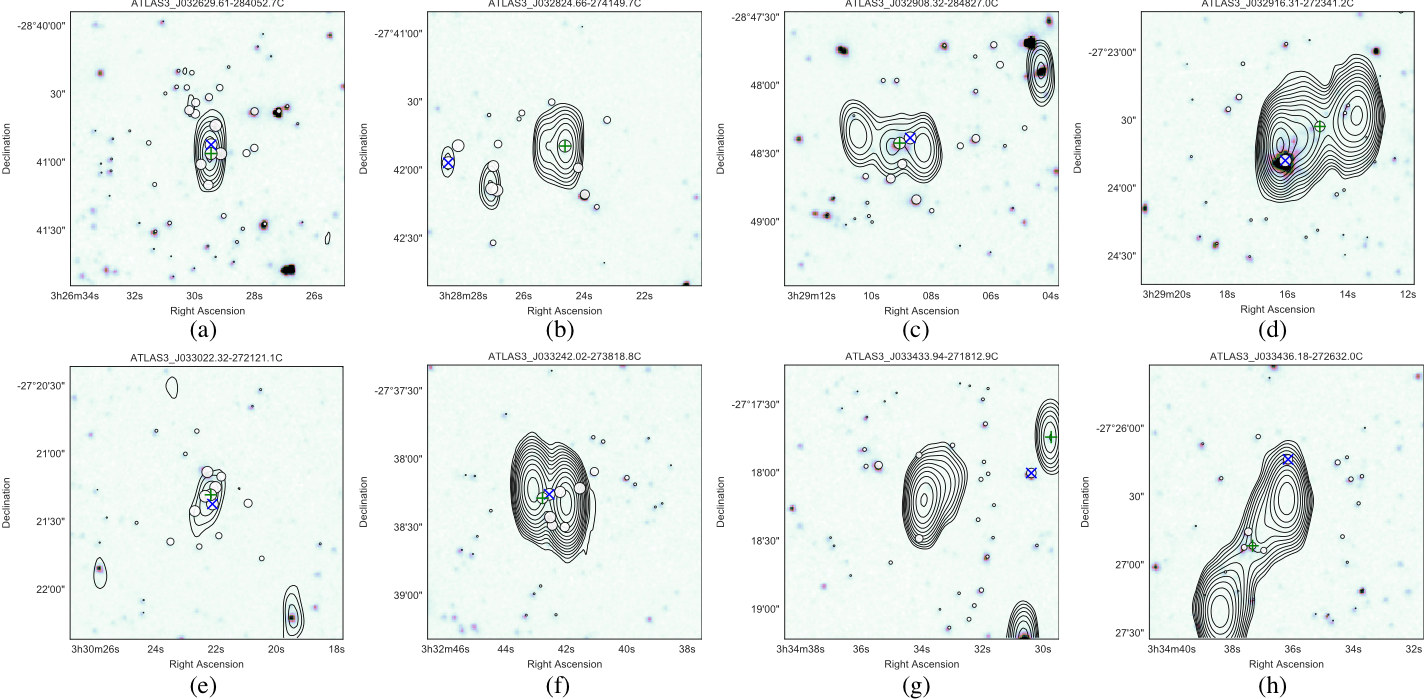
\includegraphics[width=\textwidth]{images/CNN-examples-CDFS.png}
      \caption{Radio sources in CDFS incorrectly cross-identified by a
        convolutional neural network trained on expert labels.
        (a), (e), and (f) have multiple SWIRE host galaxies very close
        together and the predicted host galaxy is close to the true host galaxy.
        (b) contains multiple radio sources, and the
        identified host likely \emph{is} a host galaxy, but not one labelled in
        the initial ATLAS data release, as it is a low flux source. In
        (c), the classifier seems to be distracted by the
        right lobe of the radio source. This may be due to the large number of
        compact objects in the training set.
        (d) and (h) show the
        classifier failing to correct cross-identify a radio double. This may be
        due to the window size (both lobes would not be visible in the radio image
        shown to the classifier) or due to the limited number of radio doubles in
        the training set. Finally,
       (g) shows the classifier failing to classify a radio
        triple. This triple extends outside the 1~arcmin radius used to select
        candidate hosts.}\label{fig:cnnexamples}
  \end{figure*}

  % \begin{figure}
  %   \centering
  %   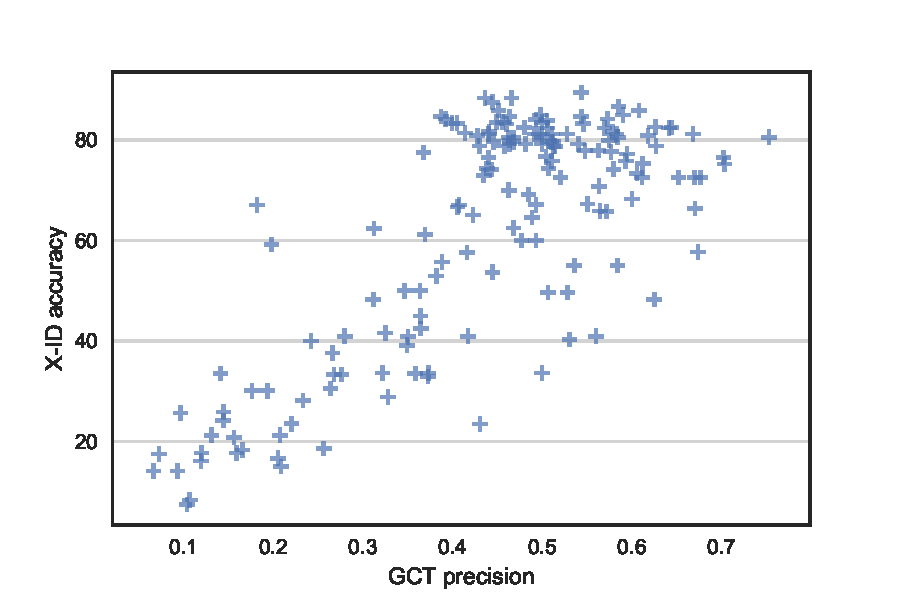
\includegraphics[width=\columnwidth]{gct-to-xid-precision.pdf}
  % \end{figure}

  % \begin{figure}
  % \centering
  % 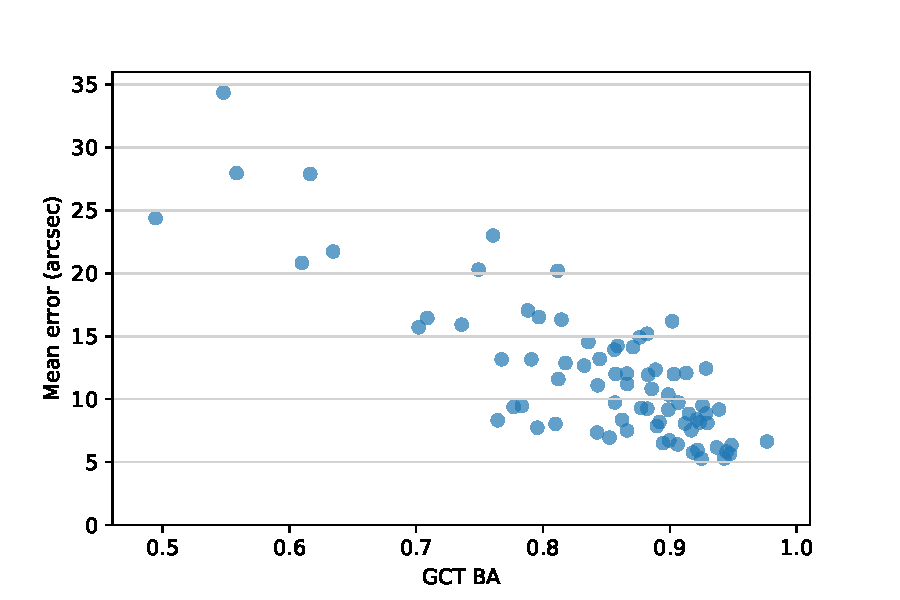
\includegraphics[width=\columnwidth]{gct-to-arcsec-error.pdf}
  % \caption{Classification balanced accuracy against average radial
  % distance between the predicted and the \citet{norris06} cross-identified
  % host on the cross-identification task.\label{fig:gct-to-arcsec-error}}
  % \end{figure}

  % \begin{figure}
  % \centering
  % 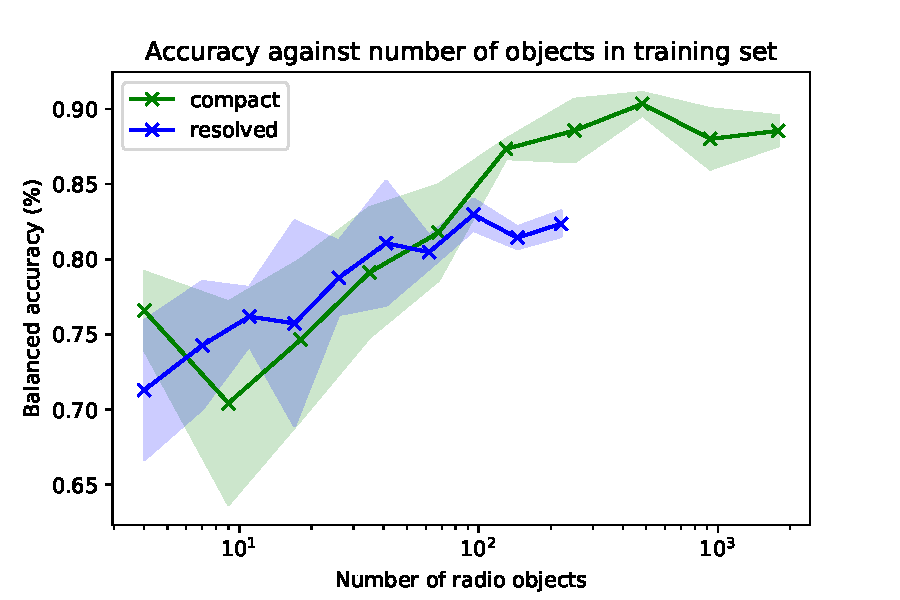
\includegraphics[width=\columnwidth]{passive.pdf}
  % \caption{Passive learning plot for the GCT. Trained and tested on RGZ.
  %   This is so that we had maximal training data --- RGZ has many more
  %   \label{fig:passive}}
  % \end{figure}

  % \begin{figure}
  % \centering
  % 
\includegraphics[width=\columnwidth]{distributions.pdf}
  % \caption{Distribution of non-image features.\label{fig:distributions}}
  % \end{figure}

  % \begin{figure}
  % \centering
  % 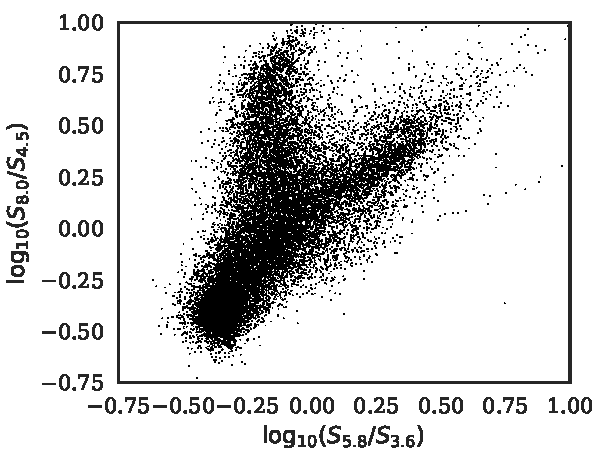
\includegraphics[width=\columnwidth]{images/swire_colour_colour.pdf}
  % \caption{Colour-colour diagram for sample of SWIRE objects in CDFS.
  %   \label{fig:colour-colour-all}}
  % \end{figure}

  % \begin{figure*}
  % \centering
  % \subfloat[\label{fig:colour-colour-norris}]{\includegraphics[width=0.45\linewidth]{images/\detokenize{swire_colour_colour_norris}.pdf}}%
  % \subfloat[\label{fig:colour-colour-rgz}]{\includegraphics[width=0.45\linewidth]{images/\detokenize{swire_colour_colour_rgz}.pdf}}\\
  % \caption{Colour-colour diagram for \protect\subref{fig:colour-colour-norris}
  %   expert-identified infrared host galaxies in CDFS and
  %   \protect\subref{fig:colour-colour-rgz} Radio Galaxy Zoo-identified infrared
  %   host galaxies in CDFS. Dots indicate the colour-colour distribution of all
  %   SWIRE objects in CDFS, and triangles indicate identified host galaxies.
  %   \label{fig:colour-colour-norris-rgz}}
  % \end{figure*}

  % \begin{figure*}
  % \centering
  % 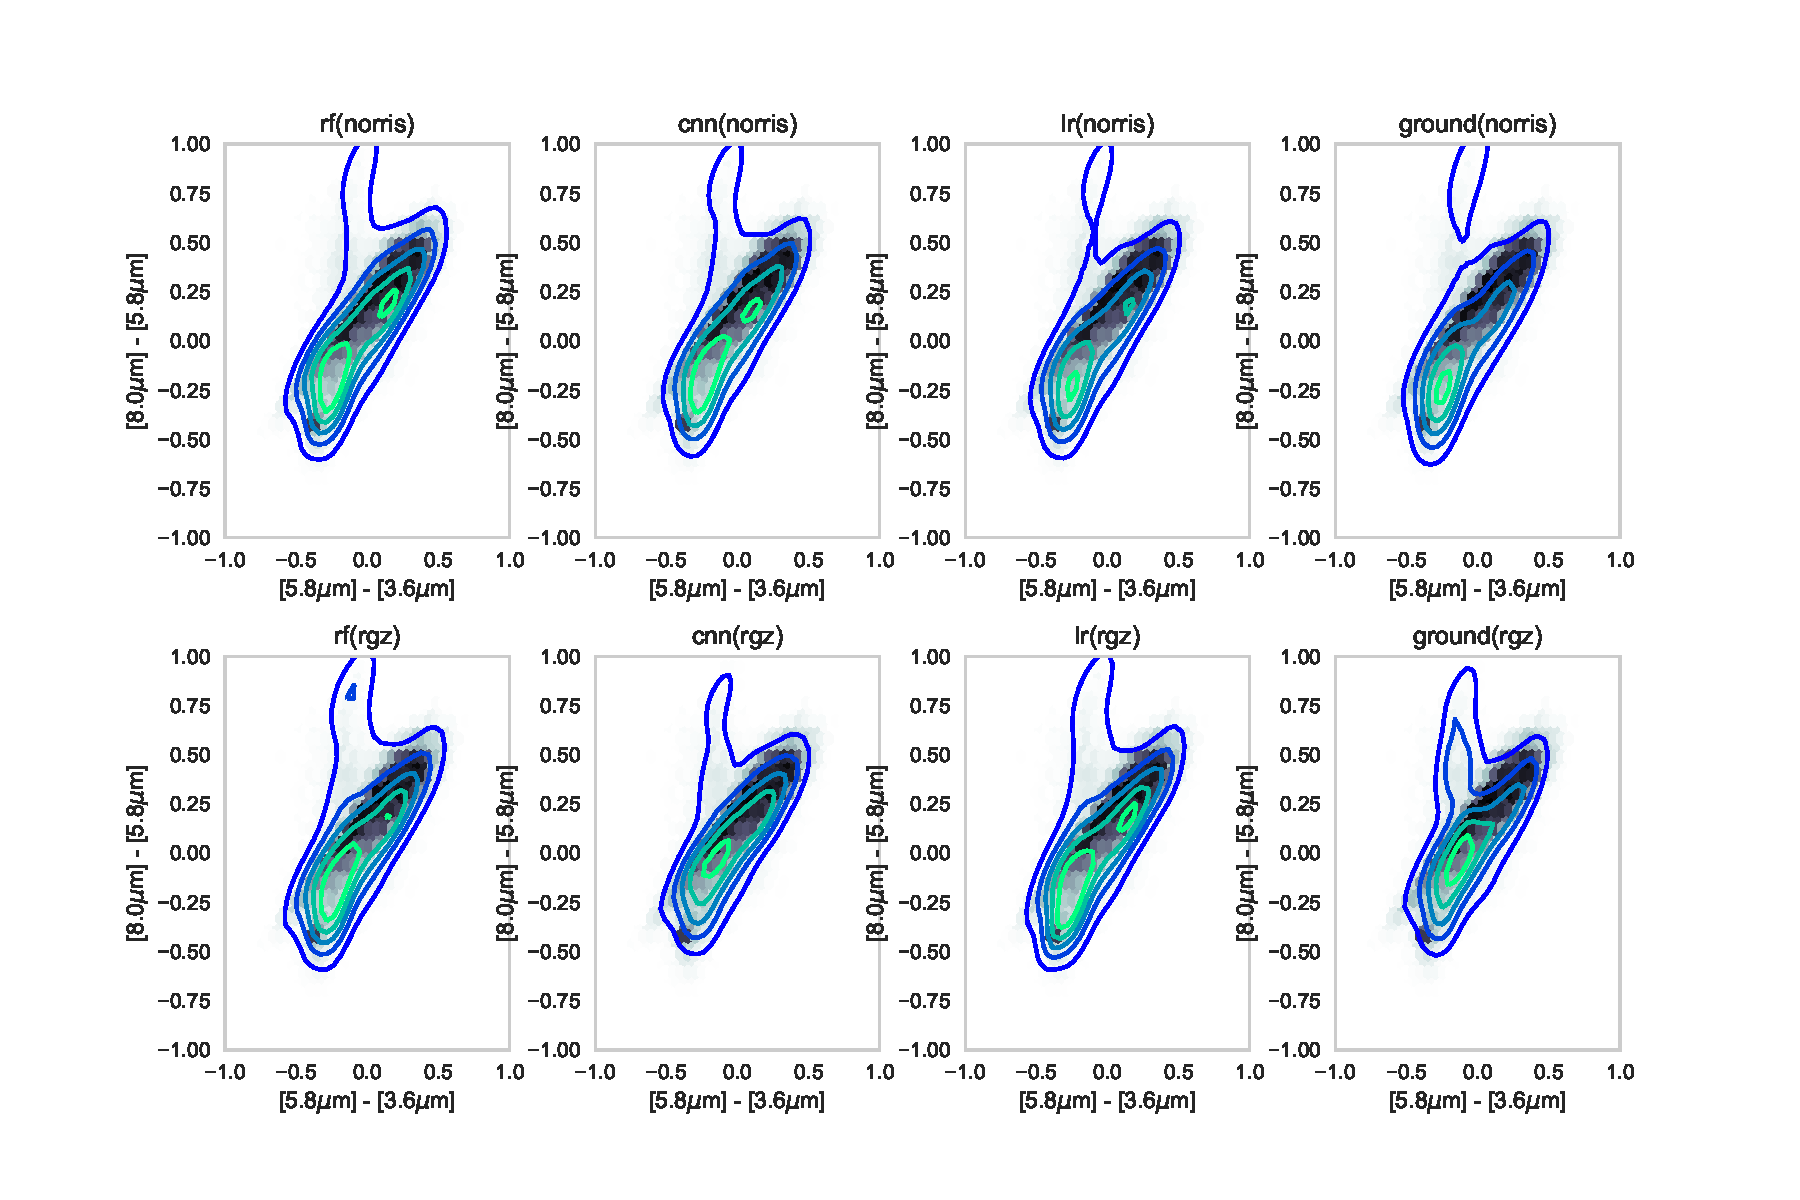
\includegraphics[width=\textwidth]{colour_colour_predictions.pdf}
  % \caption{Colour-colour diagrams for each
  % classifier.\label{fig:colour-colour}}
  % \end{figure*}

\subsection{Application to ATLAS-ELAIS}
  \label{sec:elais}

  \begin{figure}
  \centering
  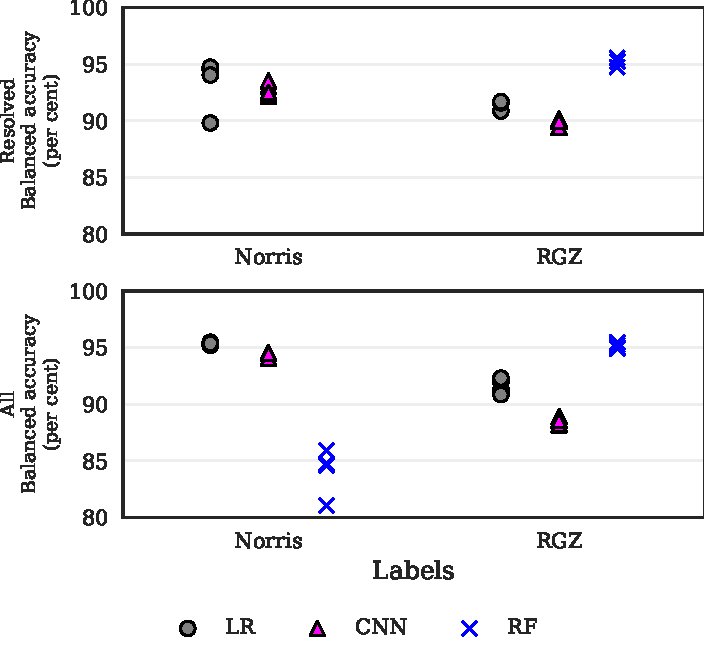
\includegraphics[width=\columnwidth]{images/elais_ba_grid.pdf}
  \caption{Balanced accuracies for each quadrant in the galaxy
    classification task on the ELAIS-S1 field. Markers and axes are as in
    \autoref{fig:ba}. The classifiers in \autoref{fig:ba} were applied to the
    whole ELAIS-S1 field, and performance was measured against ground truth
    labels from~\citet{middelberg08}. Accuracies for random forests trained on
    the expert-labelled resolved set are not shown as they were considerably
    lower than all other accuracies.
    \label{fig:elais-ba}}
  \end{figure}

  \begin{figure}
    \centering
    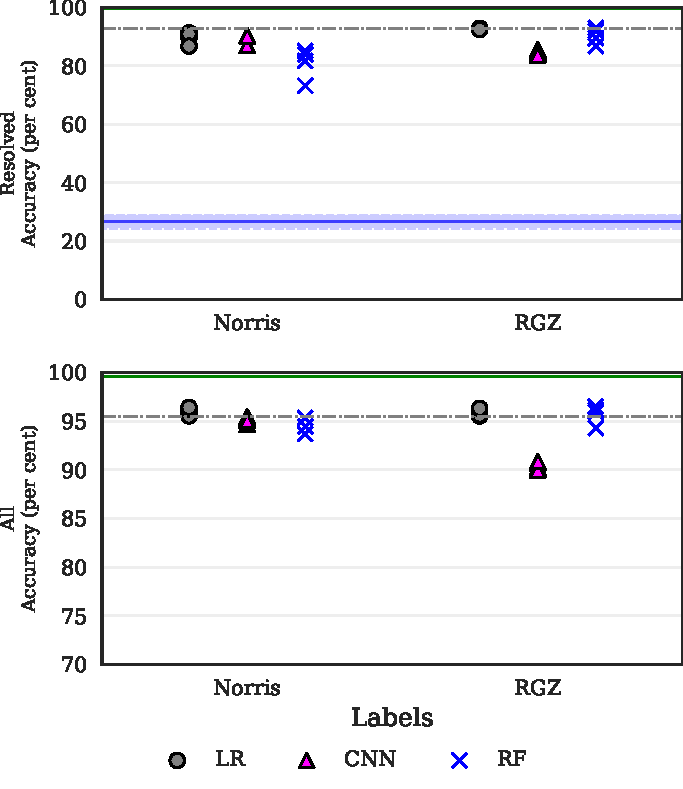
\includegraphics[width=\columnwidth]{images/elais_cross_identification_grid.pdf}
    \caption{Accuracies for each quadrant in the cross-identification
      task on the ELAIS-S1 field. Markers and axes are as in \autoref{fig:ba}.
      The classifiers in \autoref{fig:cross-id-accuracy} were applied to the
      whole ELAIS-S1 field, and performance was measured against ground truth
      labels from~\citet{middelberg08}.
      \label{fig:elais-cross-id-accuracy}}
  \end{figure}

  We applied the classifiers trained on CDFS to perform cross-identification
  on the ELAIS-S1 field. Both CDFS and ELAIS were imaged by the same radio
  telescope and to similar sensitivities and angular resolution for the ATLAS
  survey.  As ELAIS-S1 has been cross-identified with SWIRE host galaxies by
  \citet{middelberg08}, we can use these cross-identifications to derive
  another set of expert labels, and hence determine how accurate our method
  is. If our method generalises well across different parts of the sky, then
  we expect CDFS-trained classifiers applied to cross-identification in
  ELAIS-S1 to perform comparably to application to CDFS. We report the
  balanced accuracies for our classifier applied to ELAIS-S1 in
  \autoref{fig:elais-ba} and \autoref{tab:average-accuracies-elais}.
  \autoref{fig:elais-cross-id-accuracy} shows the accuracies in the
  cross-identification task on ELAIS-S1 and we list averages accuracies in
  \autoref{tab:cross-id-accuracies-elais}.

  Cross-identification results from ELAIS-S1 are similar to those for CDFS,
  showing that classifiers trained on CDFS perform reasonably well on
  ELAIS-S1. One interesting exception is that random forests trained on expert
  labels perform well on CDFS but poorly on ELAIS-S1. This is not the case for
  logistic regression or convolutional neural networks trained on expert
  labels, nor is it the case for random forests trained on Radio Galaxy Zoo.
  We hypothesise that this is because the ELAIS-S1 cross-identification
  catalogue \citep{middelberg08} labelled fainter radio components than the
  CDFS cross-identification catalogue \citep{norris06} due to noise from the
  very bright source ATCDFS\textunderscore{}J032836.53-284156.0 in CDFS.
  Classifiers trained on CDFS expert labels may thus be biased toward brighter
  radio components compared to ELAIS-S1. Radio Galaxy Zoo uses the third data
  release of ATLAS \citep{franzen15} and so classifiers trained on the Radio
  Galaxy Zoo labels may be less biased toward brighter sources compared to
  those trained on the expert labels. To test this hypothesis we tested each
  classifier against test sets with an integrated flux cutoff. A SWIRE object
  was only included in the test set for a given cutoff if it was located
  within $1'$ of a radio component with an integrated flux above the cutoff.
  The balanced accuracies for each classifier at each cutoff are shown in
  \autoref{fig:accuracies-flux}(a) and (b) and the distribution of test set
  size for each cutoff is shown in \autoref{fig:accuracies-flux}(c). (c) shows
  that ELAIS-S1 indeed has more faint objects than CDFS, with the flux cutoff
  for which the two fields reach the same test set size ($\sim 0.7$~mJy)
  indicated by the dashed vertical line on each plot. For CDFS, all
  classifiers perform reasonably well across cutoffs, with performance
  dropping as the size of the test set becomes small. For ELAIS-S1, logistic
  regression and convolutional neural networks perform comparably across all
  flux cutoffs, but random forests do not: while random forests trained on
  Radio Galaxy Zoo labels perform comparably to other classifiers across all
  flux cutoffs, random forests trained on expert labels show a considerable
  drop in performance below the dashed line.

  \begin{figure}
    \centering
    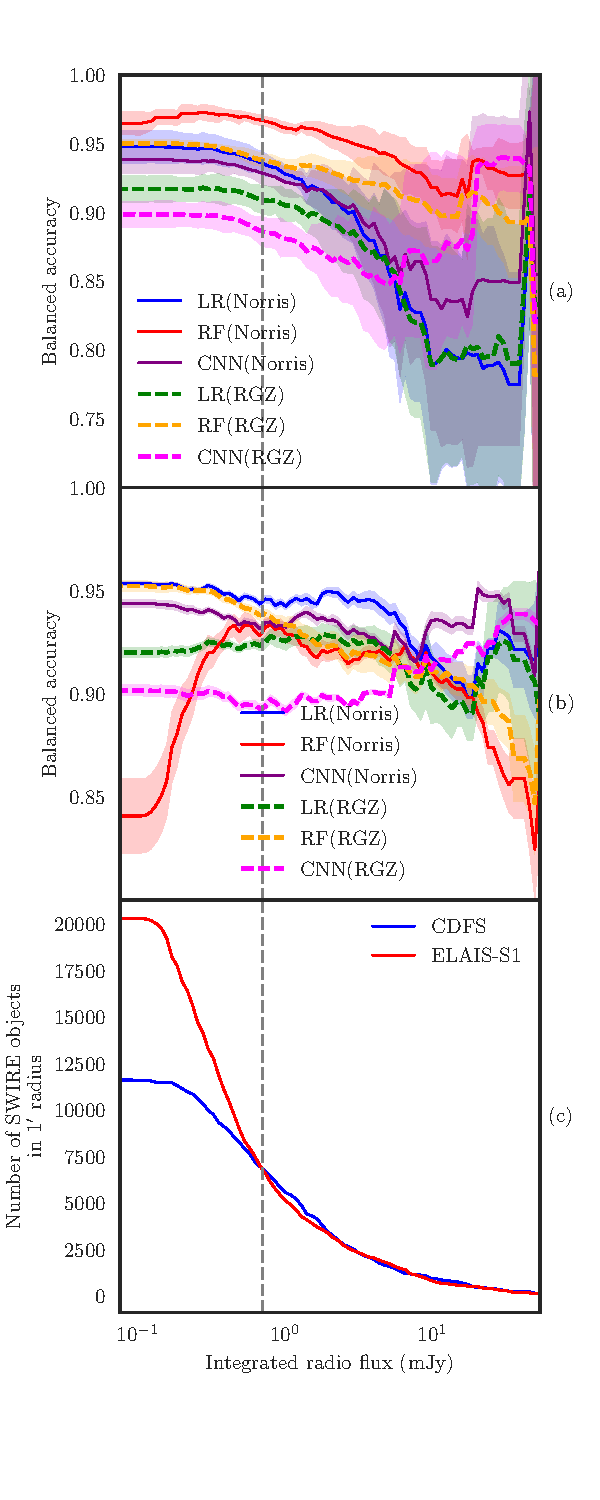
\includegraphics[width=\columnwidth, clip,
                     trim={0 2cm 0 1cm}]{images/accuracies-flux.pdf}
    \caption{(a) Balanced accuracies of classifiers trained and tested on CDFS
      with different integrated flux cutoffs for the test set. A SWIRE object
      is included in the test set if it is within $1'$ of a radio component
      with greater integrated flux than the cutoff. Different coloured lines
      indicate different classifier/training labels combinations, where LR is
      logistic regression, RF is random forests, CNN is convolutional neural
      networks, and Norris and RGZ are the expert and Radio Galaxy Zoo label
      sets respectively. Filled areas represent standard deviations across
      CDFS quadrants. (b) Balanced accuracies of classifiers trained on CDFS
      and tested on ELAIS-S1. (c) A cumulative distribution plot of SWIRE
      objects associated with a radio object with more integrated flux than
      the cutoff.}
    \label{fig:accuracies-flux}
  \end{figure}

  % \begin{figure}
  %   \centering
  %   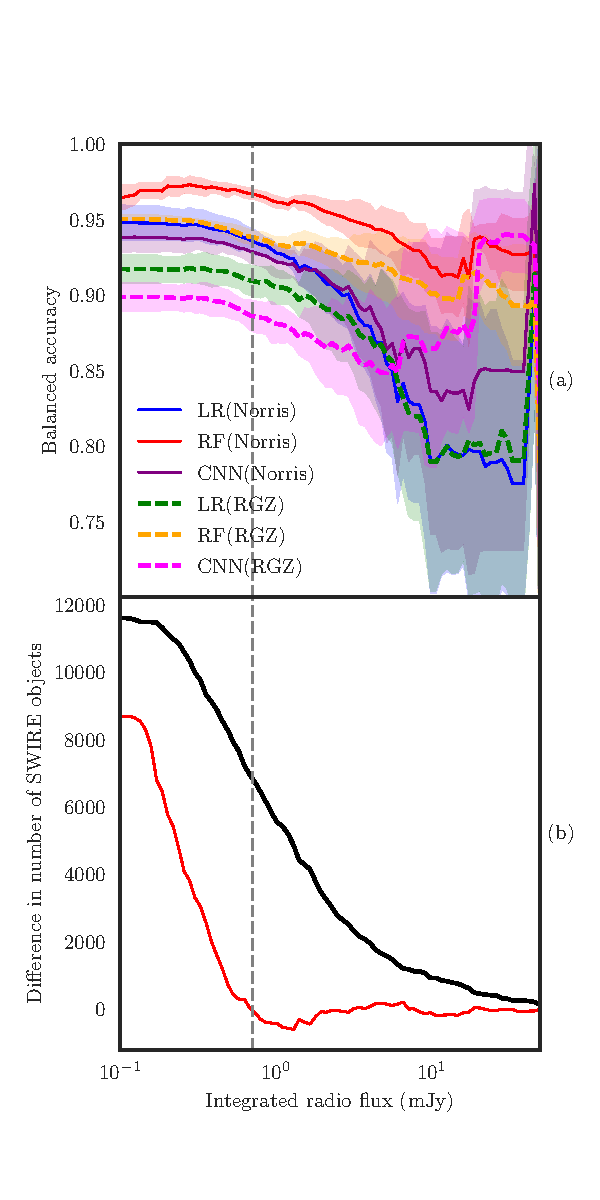
\includegraphics[width=\columnwidth]{images/cdfs-accuracies-flux.pdf}
  %   \caption{(a) Balanced accuracies of classifiers trained and tested on CDFS
  %     with different integrated flux cutoffs for the test set. A SWIRE object is
  %     included in the test set if it is within $1'$ of a radio component with
  %     greater integrated flux than the cutoff. Different coloured lines indicate
  %     different classifier/training labels combinations with definitions as in
  %     \autoref{fig:elais-accuracies-flux}. Filled areas represent standard
  %     deviations across training and testing quadrants. All classifiers perform
  %     comparably across flux cutoffs. $0.44$~mJy integrated flux is indicated by
  %     the dashed vertical line. 99\% of CDFS objects in the training and testing
  %     sets have an integrated flux exceeding this value. (b) A histogram of
  %     integrated flux for CDFS radio components. The dashed vertical line again
  %     represents the value for which 99\% of CDFS radio components have higher
  %     integrated flux.}
  %   \label{fig:cdfs-accuracies-flux}
  % \end{figure}

\section{Discussion}

  Our main result is that it is possible to cast radio host galaxy
  cross-identification as a machine learning task for which standard methods
  can be applied. These methods can then be trained with a variety of label
  sets derived from cross-identification catalogues. Future work could even
  combine multiple catalogues or physical priors to boost performance.

  The accuracies of our trained cross-identification methods generally fall
  below the best possible accuracy attainable using our approach, indicated
  by the green lines in Figures \ref{fig:cross-id-accuracy} and
  \ref{fig:elais-cross-id-accuracy}. The balanced accuracies attained by our
  binary classifiers indicate that there is significant room for improvement
  in classification. The classification accuracy can be improved by better
  model selection and more training data, particularly for convolutional
  neural networks. There is a huge variety of ways to build a convolutional
  neural network, and we have only investigated one architecture. For an
  exploration of different convolutional neural network architectures
  applied to radio astronomy, see \citet{lukic17compact}. Convolutional
  neural networks generally require more training data than other machine
  learning models and we have only trained our networks on a few hundred
  sources. We would thus expect performance on the classification task to
  greatly increase with larger training sets.

  Another problem is that of the window size used to select radio features.
  Increasing window size would increase computational expense, but provide
  more information to the models. Results are also highly sensitive to how
  large the window size is compared to the size of the radio galaxy we are
  trying to cross-identify, with large angular sizes requiring large window
  sizes to ensure that the features contain all the information needed to
  localise the host galaxy. An ideal implementation of our method would most
  likely represent a galaxy using radio images taken at multiple window
  sizes, but this is considerably more expensive.

  Larger training sets, better model selection, and larger window sizes
  would improve performance, but only so far: we would still be bounded
  above by the estimated ``perfect'' classifier accuracy. From this point,
  the performance can only be improved by improving upon our broken
  assumptions. We detailed these assumptions in \autoref{sec:limitations},
  and we will discuss here how these could be resolved. Our assumption that
  we have only one radio object in a given radius is easily broken by radio
  galaxies with large angular size, as these may overlap other radio
  objects. Source identification may solve this problem. An example of how
  source identification could help resolve the issue is to identify all
  sources, then cross-identify the galaxies in order of angular size,
  excluding previous host galaxies each time. Source identifications may
  also provide priors on the true host galaxy location: candidate hosts can
  be generated based on physical models applied to sources, and then these
  hosts can be selected from using our model. Our assumption that the host
  galaxy is contained within the search radius could be improved by
  dynamically choosing the search radius, perhaps based on the angular
  extent of the galaxy, or the redshift of candidate hosts. Finally, our
  assumption that the host galaxy is visible in infrared is technically not
  needed, as the sliding window approach we have employed will still work
  even if there are no visible host galaxies --- instead of classifying
  candidate hosts, simply classify each pixel in the radio image. The
  downside of removing candidate hosts is that we are no longer able to
  reliably incorporate host galaxy information such as colour and redshift,
  though this could be resolved by treating pixels as potentially invisible
  candidate hosts with noisy features.

  We observe that Radio Galaxy Zoo-trained methods perform comparably to
  methods trained on expert labels. This shows that the crowdsourced labels
  from Radio Galaxy Zoo will indeed provide a valuable source of training
  data for future machine learning methods in radio astronomy.

  \autoref{fig:accuracies-flux} reveals interesting behaviour of different
  classifier models at different flux cutoffs. Logistic regression and
  convolutional neural networks seem relatively independent of flux, with
  these models performing well on the fainter ELAIS-S1 sources even when
  they were trained on the generally brighter objects in CDFS. Conversely,
  random forests were sensitive to the changes in flux distribution between
  datasets. This shows that not all models behave similarly on radio data,
  and it is therefore important to investigate multiple models when
  developing machine learning methods for radio astronomy.

  Our methods can be easily incorporated into other cross-identification
  methods or used as an extra data source for source identification. This is
  because we have essentially produced a scoring function, which rates
  galaxies based on the probability that they are a host galaxy. For
  example, our method could be used to disambiguate between candidate host
  galaxies selected by model-based algorithms, or used to weight candidate
  host galaxies while a source identifier attempts to associate radio
  components. Our method can also be extended using other data sources; for
  example, information from source identification algorithms could be
  incorporated into the feature set of candidate host galaxies.

\section{Summary}

  We present a machine learning approach for cross-identification of radio
  components with their corresponding infrared host galaxy. We trained our
  methods on expert and crowdsourced cross-identification catalogues, and
  applied these methods on the CDFS and ELAIS-S1 fields of ATLAS.
  Expert-trained models generally outperformed the crowdsourced-trained
  models, but both sets of models performed comparably on the
  cross-identification task. While our cross-identification performance is not
  as high as would be ideal, we make no assumptions on the binary
  classification model used in our methods and so we expect the performance to
  be improved by further experimentation and model selection. Our method
  provides a useful framework for generalising cross-identification catalogues
  to unseen areas of the sky and can be incorporated into existing methods.
  \todo{Add recommendations and update with respect to abstract.}

%
%%%%%%%%%%%%%%%%%%%% REFERENCES %%%%%%%%%%%%%%%%%%
\bibliographystyle{mnras}
\bibliography{rgz-cdfs-ms}

%%%%%%%%%%%%%%%%%%%%%%%%%%%%%%%%%%%%%%%%%%%%%%%%%%
\clearpage
\appendix
\section{Tables of accuracies}

\cheng{need some descriptive text}

\cheng{why don't we just report the 4 raw numbers? A standard error from four values seems fishy.}

\begin{table*}
  \caption{Average balanced accuracies across quadrants shown in
    \autoref{fig:ba} for CDFS. Uncertainties represent standard
    deviations. The classifiers were trained and tested on compact
    sources, resolved sources, and all sources separately. `Labeller'
    indicates what label set the classifiers were trained on. `Norris' is
    the expert label set, `RGZ' is the Radio Galaxy Zoo label set.%, and
    %`RGZ N' is the Radio Galaxy Zoo label set with only radio sources that
    %were also labelled by experts.
    `LR' refers to logistic regression, `CNN' refers to our convolutional
    neural network, and `RF' refers to random forests.}
  \label{tab:average-accuracies}
  \begin{tabular}{llccc}
    \hline
    Labeller & Classifier & Mean `Compact' accuracy & Mean `Resolved' accuracy & Mean `All' accuracy\\
     & & (per cent) & (per cent) & (per cent)\\
    \hline
    Norris & CNN & $92.6 \pm 0.7$ & $91.2 \pm 0.5$ & $92.1 \pm 0.6$\\
     & LR & $91.6 \pm 1.0$ & $93.2 \pm 1.0$ & $93.1 \pm 1.2$\\
     & RF & $97.5 \pm 0.6$ & $90.9 \pm 4.8$ & $96.7 \pm 2.3$\\
     \\
    % RGZ N & CNN & $89.4 \pm 0.6$ & $89.6 \pm 1.3$ & $89.4 \pm 0.5$\\
    %  & LR & $89.5 \pm 0.8$ & $90.5 \pm 1.7$ & $90.2 \pm 0.8$\\
    %  & RF & $94.6 \pm 0.1$ & $95.8 \pm 0.5$ & $94.7 \pm 0.5$\\
    %  \\
    RGZ & CNN & $87.8 \pm 0.7$ & $89.2 \pm 0.7$ & $87.7 \pm 0.9$\\
     & LR & $91.4 \pm 0.8$ & $89.8 \pm 0.8$ & $90.8 \pm 1.4$\\
     & RF & $94.0 \pm 0.6$ & $94.7 \pm 0.6$ & $94.1 \pm 0.3$\\
    \hline
  \end{tabular}
\end{table*}

\begin{table}
  \caption{Average cross-identification accuracies across quadrants.
    Uncertainties represent standard deviations across quadrants and, for
    the `random' classifier, 25 random classifiers. Columns and
    classifiers as defined in \autoref{tab:average-accuracies}.  A
    `perfect' classifier reads the expert labels directly and hence
    represents the maximum attainable accuracy on the test set under our
    assumptions. A `random' classifier generates uniform random class
    probabilities and hence represents the expected minimum attainable
    accuracy with our cross-identification method.}
    \label{tab:cross-id-accuracies}
  \begin{tabular}{llcc}
  \hline
  Labeller & Classifier  & Mean `Resolved' & Mean `All' \\
   & & accuracy (per cent) & accuracy (per cent)\\
  \hline
  Norris & CNN & $61.1 \pm 15.1$ & $93.0 \pm 1.5$\\
   & LR & $66.5 \pm 6.9$ & $92.8 \pm 1.5$\\
   & RF & $67.2 \pm 5.9$ & $92.4 \pm 1.2$\\
   & Perfect & $92.1 \pm 1.5$ & $96.7 \pm 1.8$\\
   & Random & $4.7 \pm 3.9$ & $79.7 \pm 5.4$\\
   \\
  % RGZ-N & CNN & $48.6 \pm 11.5$ & $87.6 \pm 2.1$\\
  %  & LR & $64.6 \pm 11.1$ & $91.7 \pm 1.0$\\
  %  & RF & $65.8 \pm 4.7$ & $89.2 \pm 3.4$\\
  %  \\
  RGZ & CNN & $41.3 \pm 4.9$ & $86.4 \pm 2.7$\\
   & LR & $60.0 \pm 11.5$ & $92.6 \pm 1.9$\\
   & RF & $57.0 \pm 6.1$ & $87.1 \pm 2.6$\\
   \hline
  \end{tabular}
\end{table}

\begin{table*}
  \caption{Average balanced accuracies across quadrants shown in
    \autoref{fig:elais-ba} for ELAIS-S1. Uncertainties represent standard
    deviations. The classifiers were applied to compact sources, resolved
    sources, and all sources separately.}
  \label{tab:average-accuracies-elais}
  \begin{tabular}{ccccc}
    \hline
    Labeller & Classifier & Mean `Compact' accuracy & Mean `Resolved' accuracy & Mean `All' accuracy \\
     & & (per cent) & (per cent) & (per cent)\\
    \hline
    Norris & CNN & $94.8 \pm 0.2$ & $92.8 \pm 0.5$ & $94.4 \pm 0.2$ \\
     & LR & $94.6 \pm 0.4$ & $93.3 \pm 2.0$ & $95.3 \pm 0.1$ \\
     & RF & $87.4 \pm 5.6$ & $71.5 \pm 2.3$ & $86.0 \pm 2.6$ \\
     \\
    % RGZ N & CNN & $90.11 \pm 0.34$ & $91.13 \pm 0.92$ & $90.17 \pm 0.27$ \\
    %  & LR & $91.81 \pm 0.29$ & $91.94 \pm 0.53$ & $92.01 \pm 0.24$ \\
    %  & RF & $95.18 \pm 0.30$ & $95.16 \pm 0.69$ & $95.50 \pm 0.24$ \\
    %  \\
    RGZ & CNN & $88.8 \pm 0.6$ & $89.9 \pm 0.3$ & $88.5 \pm 0.3$ \\
     & LR & $93.2 \pm 0.5$ & $91.4 \pm 0.3$ & $91.6 \pm 0.6$ \\
     & RF & $94.9 \pm 0.2$ & $95.2 \pm 0.3$ & $95.1 \pm 0.2$ \\
     \hline
  \end{tabular}
\end{table*}

\begin{table}
  \caption{Average cross-identification accuracies for ELAIS-S1.
    Uncertainties represent standard deviations across classifiers trained
    on CDFS quadrants. Columns and classifiers as defined in Table
    \ref{tab:average-accuracies}.  A `perfect' classifier reads the expert
    labels directly and hence represents the maximum attainable accuracy
    under our assumptions. A `random' classifier generates uniform random
    class probabilities and hence represents the expected minimum attainable
    accuracy with our cross-identification method.}
    \label{tab:cross-id-accuracies-elais}
  \begin{tabular}{llcc}
    \hline
    Labeller & Classifier  & Mean `Resolved' & Mean `All' \\
     & & accuracy (per cent) & accuracy (per cent)\\
    \hline
    Middelberg & Perfect & $85.8 \pm 0.6$ & $92.4 \pm 0.3$\\
               & Random  & $4.7 \pm 1.0$  & $50.7 \pm 0.5$\\
     \\
    Norris & CNN     & $68.1 \pm 2.5$ & $85.6 \pm 0.7$\\
           & LR      & $79.6 \pm 0.9$ & $90.2 \pm 0.6$\\
           & RF      & $76.1 \pm 3.4$ & $90.4 \pm 1.5$\\
     \\
    % RGZ-N & CNN & $61.01 \pm 1.40$ & $78.38 \pm 0.49$\\
    %       & LR  & $75.71 \pm 1.11$ & $86.72 \pm 1.10$\\
    %       & RF  & $75.00 \pm 2.42$ & $86.96 \pm 1.80$\\
    %  \\
    RGZ & CNN & $59.1 \pm 3.2$ & $76.5 \pm 0.5$\\
        & LR  & $75.8 \pm 2.1$ & $88.3 \pm 0.8$\\
        & RF  & $75.2 \pm 2.9$ & $86.2 \pm 1.3$\\
     \hline
  \end{tabular}
\end{table}


\section{Catalogues}
  \begin{table*}
    \caption{Predicted probabilities that each object in SWIRE is a host
      galaxy. Probabilities are reported for each predictor. $C(A\ /\ B)$
      indicates the predictor using classifier model $C$, trained on label set
      $A$ on data set $B$. Ellipsis indicates columns that have been omitted.
      The omitted columns are all other combinations of classifier, label set,
      and data set. If a SWIRE object does not appear in the table, then it
      was further than 1 arcmin from an ATLAS object and hence has a predicted
      probability of zero by our assumptions. Full table electronic.}
    \label{tab:probs}
    \begin{tabular}{ccccccccccccccccccccc}
      \hline
      SWIRE & RA & Dec & CNN(Norris / All) & & RF(RGZ / Resolved) \\\hline
      SWIRE3\textunderscore{}J032559.15-284724.2 & 51.4965 & -28.7901 & 0.0001 & $\cdots$ & 0.1170 \\
      SWIRE3\textunderscore{}J032559.91-284728.9 & 51.4996 & -28.7914 & 0.0004 & $\cdots$ & 0.0000 \\
      SWIRE3\textunderscore{}J032600.02-284736.9 & 51.5001 & -28.7936 & 0.0002 & $\cdots$ & 0.0451 \\
      SWIRE3\textunderscore{}J032600.13-284637.5 & 51.5005 & -28.7771 & 0.0004 & $\cdots$ & 0.0637 \\
      SWIRE3\textunderscore{}J032600.13-284715.7 & 51.5006 & -28.7877 & 0.0014 & $\cdots$ & 0.0153 \\
      SWIRE3\textunderscore{}J032600.98-284705.4 & 51.5041 & -28.7848 & 0.0205 & $\cdots$ & 0.0000 \\
      SWIRE3\textunderscore{}J032601.03-284711.6 & 51.5043 & -28.7866 & 0.0699 & $\cdots$ & 0.0000 \\
      SWIRE3\textunderscore{}J032601.56-284131.0 & 51.5065 & -28.692 & 0.0001 & $\cdots$ & 0.0000 \\
      SWIRE3\textunderscore{}J032601.60-284207.5 & 51.5067 & -28.7021 & 0.0000 & $\cdots$ & 0.0000 \\\hline
    \end{tabular}
  \end{table*}

 \begin{table*}
    \small
    \caption{Predicted host galaxy cross-identifications for each object in
      ATLAS. Cross-identifications are reported for each predictor, with the
      predictor listed as in \autoref{tab:probs}. The cross-identification
      given by \citet{norris06} for CDFS or \citet{middelberg08} for ELAIS-S1
      is included in the `Expert' column. For CDFS, the cross-identification
      given by the Radio Galaxy Zoo consensus is included in the `RGZ' column,
      along with the corresponding consensus levels for the radio morphology
      and host cross-identification tasks \citep[see][for details on how
      consensus is calculated]{wong17}. Low radio consensus indicates that the
      component has multiple nearby components (and thus is more impacted by
      our assumption that the source is isolated), and low infrared consensus
      indicates that the host galaxy is unclear in the SWIRE image (possibly
      due to multiple nearby candidate host galaxies). Full table electronic.}
    \begin{tabular}{ccccc}
      \hline
      ATLAS & RA & Dec & Expert & RGZ \\\hline
      ATLAS3\textunderscore{}J032602.82-284708.1C & 51.511734 & -28.785575 & SWIRE3\textunderscore{}J032603.15-284708.5 & -\\
      ATLAS3\textunderscore{}J032615.49-284629.4C & 51.564555 & -28.774847 & SWIRE3\textunderscore{}J032615.41-284630.7 & SWIRE3\textunderscore{}J032615.41-284630.7\\
      ATLAS3\textunderscore{}J032615.55-280559.8C & 51.564799 & -28.099955 & SWIRE3\textunderscore{}J032615.52-280559.8 & SWIRE3\textunderscore{}J032615.52-280559.8\\
      ATLAS3\textunderscore{}J032617.35-280710.2C & 51.572279 & -28.119491 & SWIRE3\textunderscore{}J032617.89-280707.2 & SWIRE3\textunderscore{}J032617.89-280707.2\\
      ATLAS3\textunderscore{}J032625.13-280909.8C & 51.604711 & -28.152731 & SWIRE3\textunderscore{}J032625.19-280910.1 & SWIRE3\textunderscore{}J032625.19-280910.1\\
      ATLAS3\textunderscore{}J032629.10-280650.1C & 51.621251 & -28.113924 & SWIRE3\textunderscore{}J032629.13-280650.7 & SWIRE3\textunderscore{}J032626.74-280636.7\\
      ATLAS3\textunderscore{}J032629.61-284052.7C & 51.623385 & -28.681315 & SWIRE3\textunderscore{}J032629.54-284055.8 & SWIRE3\textunderscore{}J032629.54-284055.8\\
      ATLAS3\textunderscore{}J032629.92-284753.5C & 51.624653 & -28.798195 & SWIRE3\textunderscore{}J032629.81-284754.4 & SWIRE3\textunderscore{}J032629.81-284754.4\\
      ATLAS3\textunderscore{}J032630.66-283657.3C & 51.62777 & -28.615917 & SWIRE3\textunderscore{}J032630.64-283658.0 & SWIRE3\textunderscore{}J032628.56-283744.8\\
      \hline
    \end{tabular}
    \begin{tabular}{ccccccccccccccccccccccccc}
      \hline
      RGZ radio consensus & RGZ IR consensus & CNN(Norris / All) & & RF(RGZ / Resolved) \\\hline
      0.4516 & 0.3214 & SWIRE3\textunderscore{}J032602.36-284711.5 & $\cdots$ & SWIRE3\textunderscore{}J032603.60-284627.4 \\
      0.2941 & 0.8000 & SWIRE3\textunderscore{}J032615.41-284630.7 & $\cdots$ & SWIRE3\textunderscore{}J032615.41-284630.7 \\
      0.5625 & 0.8333 & SWIRE3\textunderscore{}J032615.52-280559.8 & $\cdots$ & SWIRE3\textunderscore{}J032615.52-280559.8 \\
      0.4146 & 1.0000 & SWIRE3\textunderscore{}J032617.89-280707.2 & $\cdots$ & SWIRE3\textunderscore{}J032617.89-280707.2 \\
      0.3158 & 0.6667 & SWIRE3\textunderscore{}J032625.19-280910.1 & $\cdots$ & SWIRE3\textunderscore{}J032625.19-280910.1 \\
      0.3333 & 1.0000 & SWIRE3\textunderscore{}J032629.13-280650.7 & $\cdots$ & SWIRE3\textunderscore{}J032629.13-280650.7 \\
      0.2676 & 1.0000 & SWIRE3\textunderscore{}J032629.54-284051.9 & $\cdots$ & SWIRE3\textunderscore{}J032629.54-284051.9 \\
      1.0000 & 0.8571 & SWIRE3\textunderscore{}J032629.81-284754.4 & $\cdots$ & SWIRE3\textunderscore{}J032629.81-284754.4 \\
      0.3611 & 0.7308 & SWIRE3\textunderscore{}J032630.64-283658.0 & $\cdots$ & SWIRE3\textunderscore{}J032628.56-283744.8 \\
      \hline
    \end{tabular}
    \label{tab:cids}
  \end{table*}

  The predicted probabilities for each SWIRE object are listed in \autoref{tab:probs}. A full version of the table is available electronically.  The columns are defined as follows:
  \begin{itemize}
    \item {\em Column 1}  -- SWIRE. The SWIRE object name given in \citet{surace05swire}.
    \item {\em Column 2} -- RA. The right ascension of the SWIRE object in decimal degrees (J2000).
    \item {\em Column 3} -- Dec. The declination of the SWIRE object in decimal degrees (J2000).
    \item {\em Columns 4 -- 21} -- $C(A\ /\ B)$. The predicted probability
      that the SWIRE object is a host galaxy according to classifier $C$ trained
      on subset $B$ of label set $A$. `LR' indicates logistic regression, `RF'
      indicates random forests, `CNN' indicates convolutional neural networks,
      `Norris' indicates the expert labels, and `RGZ' indicates the Radio Galaxy
      Zoo labels.
  \end{itemize}

  The predicted cross-identifications for each ATLAS object are listed in
  \autoref{tab:cids}. A full version of the table is available electronically.
  The columns are defined as follows:
  \begin{itemize}
    \item {\em Column 1}  -- ATLAS. The ATLAS object name given in \citet{franzen15}.
    \item {\em Column 2} -- RA. The right ascension of the ATLAS object in decimal degrees (J2000).
    \item {\em Column 3} -- Dec. The declination of the ATLAS object in decimal degrees (J2000).
    \item {\em Column 4} -- Expert. The expert SWIRE cross-identification.
      This is the SWIRE object associated with the ATLAS object according to
      either \citet{norris06} or \citet{middelberg08} for CDFS and ELAIS-S1,
      respectively.
    \item {\em Column 5} -- RGZ. The Radio Galaxy Zoo cross-identification.
      This is the SWIRE object associated with the ATLAS object according to
      Radio Galaxy Zoo.
    \item {\em Column 5} -- RGZ radio consensus. The percentage agreement on
      the radio source according to Radio Galaxy Zoo. Lower numbers tend to
      indicate more complex sources. For more information on how consensus is
      generated, see \citet{wong17}.
    \item {\em Column 6} -- RGZ IR consensus. The percentage agreement on
      the host galaxy cross-identification according to Radio Galaxy Zoo.
      Lower numbers tend to indicate sources that are harder to
      cross-identify. For more information on how consensus is generated, see
      \citet{wong17}.
    \item {\em Columns 7 -- 25} -- $C(A\ /\ B)$. The predicted
      cross-identification according to classifier $C$ trained on subset $B$
      of label set $A$. `LR' indicates logistic regression, `RF' indicates
      random forests, `CNN' indicates convolutional neural networks, `Norris'
      indicates the expert labels, and `RGZ' indicates the Radio Galaxy Zoo
      labels.
  \end{itemize}

% Don't change these lines
\bsp	% typesetting comment
\label{lastpage}
\end{document}
